% ---------------------------------------------------------------------
% EG author guidelines plus sample file for EG publication using LaTeX2e input
% D.Fellner, v1.17, Sep 23, 2010


\title[Peridynamics-Based Fracture Animation for Elastoplastic Solids]%
      {Peridynamics-Based Fracture Animation for Elastoplastic Solids}

% for anonymous conference submission please enter your SUBMISSION ID
% instead of the author's name (and leave the affiliation blank) !!
\author[W. Chen et al.]{W. Chen, F. Zhu, J. Zhao,
  S. Li, G. Wang}

%\author[D. Fellner \& S. Behnke]
%       {D.\,W. Fellner\thanks{Chairman Eurographics Publications Board}$^{1,2}$
%        and S. Behnke$^{2}$
%%        S. Spencer$^2$\thanks{Chairman Siggraph Publications Board}
%        \\
%% For Computer Graphics Forum: Please use the abbreviation of your first name.
%         $^1$TU Darmstadt \& Fraunhofer IGD, Germany\\
%         $^2$Institut f{\"u}r ComputerGraphik \& Wissensvisualisierung, TU Graz, Austria
%%        $^2$ Another Department to illustrate the use in papers from authors
%%             with different affiliations
%       }

% ------------------------------------------------------------------------

% if the Editors-in-Chief have given you the data, you may uncomment
% the following five lines and insert it here
%
% \volume{27}   % the volume in which the issue will be published;
% \issue{1}     % the issue number of the publication
% \pStartPage{1}      % set starting page


%-------------------------------------------------------------------------
\begin{document}

\teaser{
 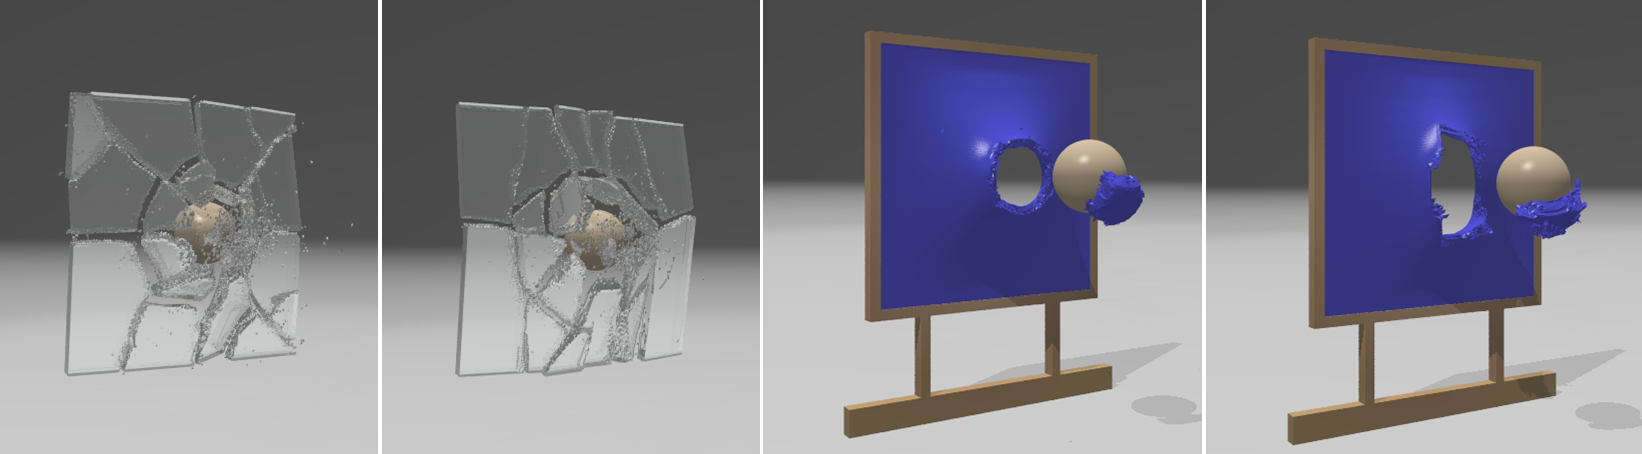
\includegraphics[width=\linewidth]{../figs/demo_impact.png}
 \centering
  \caption{ A sphere shoots through walls made of different materials, causing varied fracture behaviors. From left to right: isotropic brittle fracture, anisotropic brittle fracture, isotropic ductile fracture, anisotropic ductile fracture.}
\label{fig:1}
}

\maketitle

\begin{abstract}
In this paper, we exploit the use of peridynamics theory for graphical animation of material deformation and fracture. We present a new meshless framework for elastoplastic constitutive modeling that contrasts with previous approaches in graphics. Our peridynamics-based elastoplasticity model represents deformation behaviors of materials with high realism. We validate the model by varying the material properties and performing comparisons with FEM simulations. The integral-based nature of peridynamics makes it trivial to model material discontinuities, which outweighs differential-based methods in both accuracy and ease of implementation. We propose a simple strategy to model fracture in the setting of peridynamics discretization. We demonstrate that the fracture criterion combined with our elastoplasticity model could realistically produce ductile fracture as well as brittle fracture. Our work is the first application of peridynamics in graphics that could create a wide range of material phenomena including elasticity, plasticity, and fracture. The complete framework provides an attractive alternative to existing methods for producing modern visual effects.
\begin{keywords}
peridynamics, fracture, elastoplasticity
\end{keywords}
\begin{classification} % according to http://www.acm.org/class/1998/
\CCScat{Computer Graphics}{I.3.7}{Three-Dimensional Graphics and Realism}{Animation}
\end{classification}

\end{abstract}

%-------------------------------------------------------------------------
\section{Introduction}

The simulation of deformable materials has been an important research topic in computer graphics for decades, since the early work by Terzopoulos and colleagues \cite{Terzopoulos:1987:EDM:37402.37427}. One of the strongest driving forces behind the active research is the persistently growing need for higher realism from the visual effects industry. Materials in the real world exhibit complex behaviors, such as coupled elastoplastic deformations, fracture, etc. The complicated material behaviors are difficult to replicate by any single method despite the numerous ones that have been developed thus far. Existing approaches generally excel at some phenomena but would stumble (if not fail) at others. For instance, mesh-based methods \cite{Muller:2004:IVM:1006058.1006087,Irving:2004:IFE:1028523.1028541,Teran:2005:RQF:1073368.1073394,Sifakis:2012:FSD:2343483.2343501} are a good choice to simulate elastic deformations whereas not preferred for phenomena that involve topological changes. Particle-based methods \cite{Muller:2003:PFS:846276.846298,Pauly:2005:MAF:1073204.1073296,Stomakhin:2013:MPM:2461912.2461948} are considered suitable for modeling topological changes, however the inherent loss of connectivity information would cause undesirable numerical fracture \cite{Liu:2011:AKM:2065362.2066108, Zhu:2016MPM} while simulating large deformations.

We build on recent developments of peridynamics theory in the computational physics community \cite{Silling2000,silling2007peridynamic,mitchell2011nonlocal, emmrich2013peridynamics,madenci2014peridynamic} and propose a novel framework for graphical animation of varied deformation behaviors and fracture. Our aim is to enrich available options of simulation techniques for easier and better animation production. Peridynamics was first adopted to animation applications by Levine et al. \cite{Levine:2015:PPS:2849517.2849526} where they described a simple spring-mass system to handle brittle fracture of solids. In contrast, we handle elastoplasticiy, brittle fracture, and ductile fracture in a single framework. To this end, we propose several novel contributions in this work. We first present an elastoplastic constitutive model in the peridynamics-based framework with simple extension to anisotropy, and the model is validated against results produced by FEM. Furthermore, we show that both brittle and ductile fracture phenomena can be naturally represented with nearly no effort by integrating a simple fracture criterion into this material model. This is due to the integral-based formulation of peridynamics, in which forces at a material point are computed by gathering contributions from all material points in its interaction range through integration. On the other hand, methods based on classical continuum mechanics formulate force computations with partial differential equations that fail to be applicable directly on singularities such as a crack. This feature makes our peridynamics-based framework more attractive over existing approaches for producing animations that involve fracture. Lastly, our method is simple to implement and trivially parallelizable, providing a useful alternative to previous methods for animation production.

%-------------------------------------------------------------------------
\section{Related Work}

A large body of literature has been devoted to physical simulation of natural phenomena as a result of active research. A complete literature review is beyond the scope of this paper. In the following we comment only on the representative works most related to ours.

\noindent{\textbf{Elastoplasticity Animation}}~The modeling of deformable plasticity in graphics dates back to the pioneering work by Terzopoulos and Fleischer \cite{Terzopoulos:1988:MID:378456.378522}. O'Brien and colleagues \cite{O'Brien:2002:GMA:566654.566579} incorporated a similar additive plasticity model into a finite element simulation to animate ductile fracture. The strain measure was decomposed into two components, where one is due to elastic deformation and the other due to plastic deformation. M\"{u}ller et al. \cite{Muller:2004:PBA:1028523.1028542} applied this model in their point-based animation framework and simulated plastic behaviors of objects.  Irving et al. \cite{Irving:2004:IFE:1028523.1028541} presented a multiplicative formulation of plasticity and pointed out that their model was better handling finite plastic deformation than the additive one. In contrast to the additive model, they decomposed the deformation gradient into two components through multiplication. The multiplicative model was extensively used by later works to animate phenomena that involve plasticity. Bargteil et al. simulated large viscoplastic flow\cite{Bargteil:2007:FEM:1276377.1276397}, Gerszewski and his colleagues animated elastoplastic solids\cite{Gerszewski:2009:PMA:1599470.1599488}, and Stomakhin et al. modeled plasticity of snow\cite{Stomakhin:2013:MPM:2461912.2461948}, just to name a few. Unfortunately, neither of the above plasticity models applies in the peridynamics framework because there is no concept of strain nor deformation gradient in the integral-based formulation. As a result, we present a new constitutive model for peridynamics in this work to animate elastoplastic solids.

\noindent{\textbf{Fracture Animation}}~Numerous methods have been proposed on fracture animation \cite{muguercia2014fracture,Wu:2015:SPB:2858852.2858866} because the stunning phenomenon of fracture and failure is an indispensable visual element in animated movies and video games. Early approaches use simple schemes to model fracture, such as the finite difference method \cite{Terzopoulos:1988:MID:378456.378522}, the mass-spring system \cite{Norton:1991:AFP:115244.115248}, and the mass-point constraint system\cite{smith2001fast}. O'Brien and colleagues \cite{O'Brien:1999:GMA:311535.311550} adopted techniques from continuum mechanics and presented a FEM-based method to simulate brittle fracture of solids. They later extended their method to ductile fracture by incorporating a plasticity model\cite{O'Brien:2002:GMA:566654.566579}. M\"{u}ller et al. \cite{Muller2001} employed a quasi-static finite element analysis to animate brittle fracture of stiff materials undergoing collisions. Parker et al. \cite{Parker:2009:RDF:1599470.1599492} presented some useful techniques for real-time simulation of fracture in game environment. One major issue in FEM-based methods is the generation of fracture patterns on meshes, which could alter the underlying mesh topology. Early methods typically made use of simple separation along mesh element boundaries \cite{Norton:1991:AFP:115244.115248,Mazarak:1999:AEO:351631.351688,smith2001fast,Muller2001} or even element deletion \cite{forest2002removing}. Mesh subdivision prior to splitting could somewhat increase the available geometric details \cite{Mor:2000:MST:646923.710372,Bielser:2000:ISS:826029.826523}, whereas this tended to introduce elements with poor aspect ratios. Allowing failure along more arbitrary paths could generate more geometrically rich fracture patterns \cite{Neff:1999:VMB:351631.351686,O'Brien:1999:GMA:311535.311550,O'Brien:2002:GMA:566654.566579}, albeit at the expense of complicated re-meshing. Molino et al. \cite{Molino2004} proposed a virtual node algorithm to avoid the complexity of re-meshing, where elements were duplicated into partially filled counterparts with virtual nodes. The virtual node algorithm was frequently used by subsequent works on fracture animation \cite{Bao:2007:FRM:1263129.1263275} and mesh cutting \cite{Sifakis:2007:ACD:1272690.1272701,Wang:2015:AVN:2849517.2849531} due to its simplicity compared to re-meshing methods. Kaufmann et al. \cite{Kaufmann:2009:ETD:1531326.1531356} adapted the extended finite element method (XFEM) that enriches approximation by custom-designed basis functions, instead of actual/virtual element cutting.
Other representative mesh-based methods resorted to modal analysis \cite{glondu2013real} and pure geometric mesh decompositions \cite{Muller:2013:RTD:2461912.2461934,Schvartzman:2014:FAB:2556700.2556713} for real-time brittle fracture. Most recently, several works explored the boundary element method for rigid body fracture \cite{Zhu:2015:SRB:2809654.2766942,Hahn:2015:HBF:2809654.2766896} where only surface meshes were employed for both representation and computation.

In contrast to mesh-based approaches, meshless methods are generally considered as a better solution for animating topological changes. Based on the moving least square (MLS) meshless framework by M\"{u}ller et al. \cite{Muller:2004:PBA:1028523.1028542}, Pauly and colleagues \cite{Pauly:2005:MAF:1073204.1073296} developed a novel meshless method for fracture animation of elastoplastic solids. Steinemann et al. \cite{Steinemann:2009:SMD:1651926.1652002} employed surface mesh representation in meshless framework and presented a novel surface tracking technique to efficiently split the meshless deforming objects. Inspired by the rigid body assumption for simulating brittle fracture, Liu et al. \cite{Liu:2011:MSB:1970281.1970303} employed quasi-static analysis in a meshless local Petrov-Galerkin framework. Stomakhin et al. modeled the fracture of snow using a meshless material point method \cite{Stomakhin:2013:MPM:2461912.2461948}. Hegemann et al. \cite{Hegemann:2013:LSM:2485895.2485908} combined a level set based mesh embedding technique with the material point method to animate dynamic ductile fracture.

\noindent{\textbf{Peridynamics}}~The peridynamics theory was first proposed by Silling \cite{Silling2000} as a nonlocal reformulation of classical solid mechanics. It contrasts with classical (local) theory in that the state of a material point is influenced by not necessarily the material points located in its immediate vicinity, but also those over long distances. The governing equations of the peridynamics theory are spatial integral equations instead of partial differential equations. The theory was further developed by subsequent works \cite{silling2007peridynamic,emmrich2013peridynamics}, and its applications to the engineering field such as multi-scale material modeling \cite{askari2008peridynamics,silling2014hierarchical} and fracture modeling \cite{askari2006peridynamic,silling2010crack,silling2014peridynamic} were studied. A comprehensive review of the research literature in the computational physics community is beyond our scope, we refer the readers to the book by Madenci and Oterkus \cite{madenci2014peridynamic}.  Levine et al. \cite{Levine:2015:PPS:2849517.2849526} first introduced peridynamics to graphics for fracture animation. Their method was limited to brittle fracture of isotropic elastic materials with a single Poisson ratio of 0.25. Our work, on the other hand, is a complete framework that models elastoplasticity and anisotropy under various parameter settings, representing brittle and ductile fracture with high realism.

%-------------------------------------------------------------------------
\section{Background}\label{section:3}

\begin{figure}[t]
  \centering
  %\mbox{} \hfill
  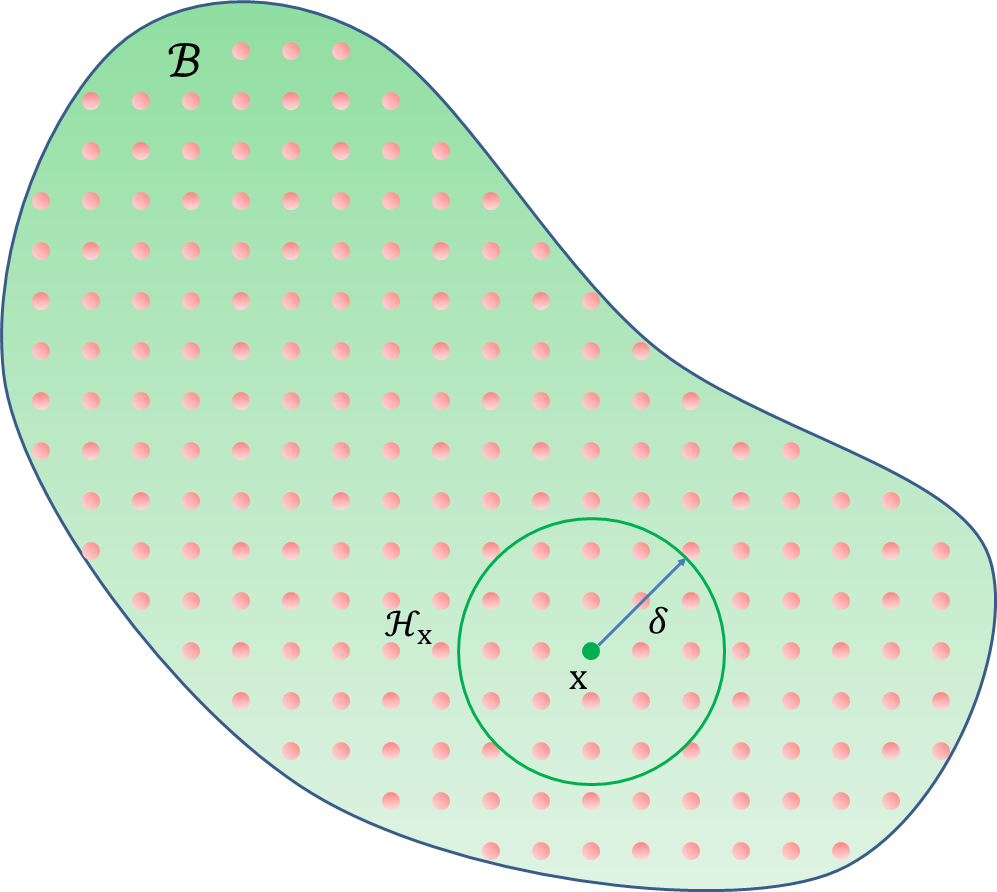
\includegraphics[width=0.7\linewidth, bb=0 0 440 355]{../figs/peridynamics_circle.png}
  \caption{\label{fig:2}
  Illustration of peridynamics discretization. A continuum is represented as particles (pink dots), and any particle (green dot) interacts with the particles within its horizon (green circle).
}
\end{figure}
In the peridynamics theory, any material point $\mathbf{x}$ interacts with other material points within a distance $\delta$. The distance $\delta$ is called the \textbf{horizon} of $\mathbf{x}$, and the material points within the horizon are referred as its \textbf{family}, $H_\mathbf{x}$. There are infinite number of family members for a material point before discretizing the continuum into discrete particles. Figure~\ref{fig:2} is an illustration of the peridynamics discretization with particles. It seems analogous to other meshless \nobreak{methods} based on classical theory \cite{Muller:2003:PFS:846276.846298,Muller:2004:PBA:1028523.1028542}, and the \nobreak{difference} lies in the scale of interaction radius $\delta$. In the case of the classical (local) continuum model, the state of a particle is influenced by only particles in its immediate vicinity. For case of the peridynamics theory, however, the state of a particle is influenced by particles within a region of finite radius. The peridynamics theory is thus referred as a nonlocal theory. As the radius becomes infinitely large, the peridynamics theory becomes the continuous version of the molecular dynamics model. As the radius becomes smaller, it becomes the continuum mechanics model. Therefore, the peridynamics model establishes a connection between the continuum mechanics and molecular dynamics models.

Our motivation for choosing peridynamics is that it is more favorable to handle material discontinuities, such as cracks.
%This is due to its formulation of governing equations as spatial integral equations, which stands in contrast to the partial differential equations used in the classical formulations.
This benefit inherently from an integral force formulation of its governing equations, which stands in contrast to the partial differential equations used in the classical formulations.
As we know, spatial derivatives are not well defined at discontinuities. Therefore, special treatment is generally required for fracture modeling in existing methods that are based on classical continuum mechanics. For instance, the mesh-based methods \cite{O'Brien:1999:GMA:311535.311550,O'Brien:2002:GMA:566654.566579} employed re-meshing operations and the meshless method by Pauly et al. \cite{Pauly:2005:MAF:1073204.1073296} altered the particle weight functions. The peridynamics governing equations remain valid at discontinuities, and material damage is represented as part of the peridynamics constitutive model. These attributes permit fracture initiation and propagation to be modeled with arbitrary paths in the peridynamics framework.

In peridynamics, the governing equation at any point $\mathbf{x}$ is \nobreak{formulated} in integral form as below:
\begin{equation}
\rho\ddot{\mathbf{u}}(\mathbf{x}) = \int_{H_\mathbf{x}}[\mathbf{T}<\mathbf{x}'-\mathbf{x}> - \mathbf{T}<\mathbf{x}-\mathbf{x}'>]dH+\mathbf{b}(\mathbf{x}),
\label{eq:1}
\end{equation}
where $\rho$ is the mass density, $\mathbf{u}$ denotes the displacement, $\mathbf{b}$ is the external loads due to gravity and impact forces, and $\mathbf{x}'$ is one material point that belongs to the family $H_{\mathbf{x}}$ of $\mathbf{x}$. $\mathbf{T}<\mathbf{x}'-\mathbf{x}>$ and $\mathbf{T}<\mathbf{x}-\mathbf{x}'>$ are two essential terms in which the constitutive laws of materials are encoded. $\mathbf{T}<\mathbf{x}'-\mathbf{x}>$ represents the internal force density exerted by $\mathbf{x'}$ on $\mathbf{x}$, and $\mathbf{T}<\mathbf{x}-\mathbf{x}'>$ is the other way around. The two terms both appear in the governing equation to enforce the Newton's third law, and similar strategy was employed in SPH methods\cite{Muller:2003:PFS:846276.846298}. The angle brackets representation $<\cdot>$ was defined by Silling et al. \cite{silling2007peridynamic} as a function inside the family $H_\mathbf{x}$, which they called as a \textbf{state}. Please note the integral form of the equation, which is the key difference between peridynamics and classical theory. The entire framework is built on displacements $\mathbf{u}$ instead of their spatial derivatives, thereby making discontinuity modeling trivial. With particle discretization, the integration within $H_\mathbf{x}$ is represented as summation over family particles:
\begin{equation}
\rho\ddot{\mathbf{u}}(\mathbf{x}) = \sum_{\mathbf{x}'\in H_\mathbf{x}}[\mathbf{T}<\mathbf{x}'-\mathbf{x}> - \mathbf{T}<\mathbf{x}-\mathbf{x}'>]V_{\mathbf{x}'}+\mathbf{b}(\mathbf{x}),
\label{eq:1_sup}                    
\end{equation}
with $V_\mathbf{x}'$ as the volume of particle $\mathbf{x}'$.

%-------------------------------------------------------------------------
\section{Elastoplastic Model}

In this section we describe our constitutive model for peridynamics in detail. We start with the basic isotropic elastic model, then plasticity is incorporated, and finally we extend the model with anisotropy.

\subsection{Isotropic Elasticity}\label{section:4.1}

As is discussed in Section~\ref{section:3}, the key to peridynamics-based constitutive modeling is the design of proper internal force density $\nobreak{\mathbf{T}<\cdot>}$. Silling et al.\cite{silling2007peridynamic} showed that peridynamic constitutive models can be designed to match many hyperelastic constitutive models under the classical elasticity theory. We derive our model based on the model described by Madenci and Oterkus \cite{madenci2014peridynamic}, which matches the isotropic linear elasticity model in classical theory. The elastic internal force density exerted by particle $j$ on particle $i$ is defined as below:
\begin{equation}
\mathbf{T}_i<\mathbf{x}_j-\mathbf{x}_i> = \frac{1}{2}A\frac{\mathbf{y}_j-\mathbf{y}_i}{|\mathbf{y}_j-\mathbf{y}_i|},
\label{eq:2}
\end{equation}
where $\mathbf{x}$ and $\mathbf{y}$ denote the positions of particles before and after deformation respectively. The direction of the force density is along the deformed bond between the particles given by $\frac{\mathbf{y}_j-\mathbf{y}_i}{|\mathbf{y}_j-\mathbf{y}_i|}$. $A$ is a scalar that represents the force magnitude, and it is composed of two terms by addition $A = A_{dil} + A_{dev}$, namely the dilatation term $A_{dil}$ and the deviatoric term $A_{dev}$.

The dilatation term $A_{dil}$ is due to the dilatation part of \nobreak{deformation}, i.e., volume change without any shape distortion. It is defined as:
\begin{equation}
A_{dil}=4\omega_{ij}a\frac{\mathbf{y}_j-\mathbf{y}_i}{|\mathbf{y}_j-\mathbf{y}_i|}\cdot\frac{\mathbf{x}_j-\mathbf{x}_i}{|\mathbf{x}_j-\mathbf{x}_i|}\theta_i,
\label{eq:3}
\end{equation}
where $a$ is a peridynamics material parameter and $\omega_{ij}$ is the weight function between particle $i$ and particle $j$. For isotropic materials $\omega_{ij}$ is monotonically decreasing with respect to the distance between particles:
\begin{equation}
\omega_{ij} = \frac{\delta}{|\mathbf{x}_j-\mathbf{x}_i|}.
\label{eq:4}
\end{equation}
Note that $\omega_{ij}$ is defined in the material space, therefore can be precomputed. The term $\theta_i$ measures the dilatation at particle $i$, which is defined with respect to the stretch of all bonds between particle $i$ and its family:
\begin{equation}
\theta_i = \frac{9}{4\pi\delta^4}\sum_{k=1}^N\omega_{ik}s_{ik}\frac{\mathbf{y}_k-\mathbf{y}_i}{|\mathbf{y}_k-\mathbf{y}_i|}\cdot(\mathbf{x}_k-\mathbf{x}_i)V_k,
\label{eq:5}
\end{equation}
where $N$ represents the number of family points $k$ for point $i$, and $V_k$ are their volumes. The stretch $s_{ik}$ of the bond  between particles is defined as:
\begin{equation}
s_{ik}=\frac{|\mathbf{y}_k-\mathbf{y}_i|}{|\mathbf{x}_k-\mathbf{x}_i|} -1.
\label{eq:6}
\end{equation}

The deviatoric term $A_{dev}$ is a result of distortion that does not cause change in volume. It is defined with respect to the deviatoric component of bond extension:
\begin{equation}
A_{dev}=4\omega_{ij}b(e_{ij}-\frac{\delta}{4}\frac{\mathbf{y}_j-\mathbf{y}_i}{|\mathbf{y}_j-\mathbf{y}_i|}\cdot\frac{\mathbf{x}_j-\mathbf{x}_i}{|\mathbf{x}_j-\mathbf{x}_i|}\theta_i),
\label{eq:7}
\end{equation}
where $b$ is a material parameter. We denote $e_{ij} = |\mathbf{y}_j-\mathbf{y}_i|-|\mathbf{x}_j-\mathbf{x}_i|$ as the extension of the bond between particle $i$ and particle $j$. The term in brackets of Equation~\ref{eq:7} is the deviatoric component of bond extension $e_{ij}^d$:
\begin{equation}
e_{ij}^d = e_{ij}-\frac{\delta}{4}\frac{\mathbf{y}_j-\mathbf{y}_i}{|\mathbf{y}_j-\mathbf{y}_i|}\cdot\frac{\mathbf{x}_j-\mathbf{x}_i}{|\mathbf{x}_j-\mathbf{x}_i|}\theta_i.
\label{eq:8}
\end{equation}
Intuitively, $e_{ij}^d$ is constructed by removing the dilatation component of bond extension from the total bond extension $e_{ij}$.

In summary, the behavior of our isotropic elastic model is controlled by two material parameters $a$ and $b$. The model is equivalent to the isotropic linear elasticity model in classical theory, please refer to the supplementary document for elaborated derivation. Here we directly provide the conversion between the material parameters in this model and those from continuum mechanics:
\begin{equation}
a = \frac{9\kappa}{8\pi\delta^4} \qquad b = \frac{15\mu}{2\pi\delta^5},
\label{eq:9}
\end{equation}
where $\kappa$ and $\mu$ denote the bulk modulus and the shear modulus respectively. In Figure~\ref{fig:3} we demonstrate an example of the hyperelastic deformations animated with our model.
\begin{figure}[t]
  \centering
  %\mbox{} \hfill
  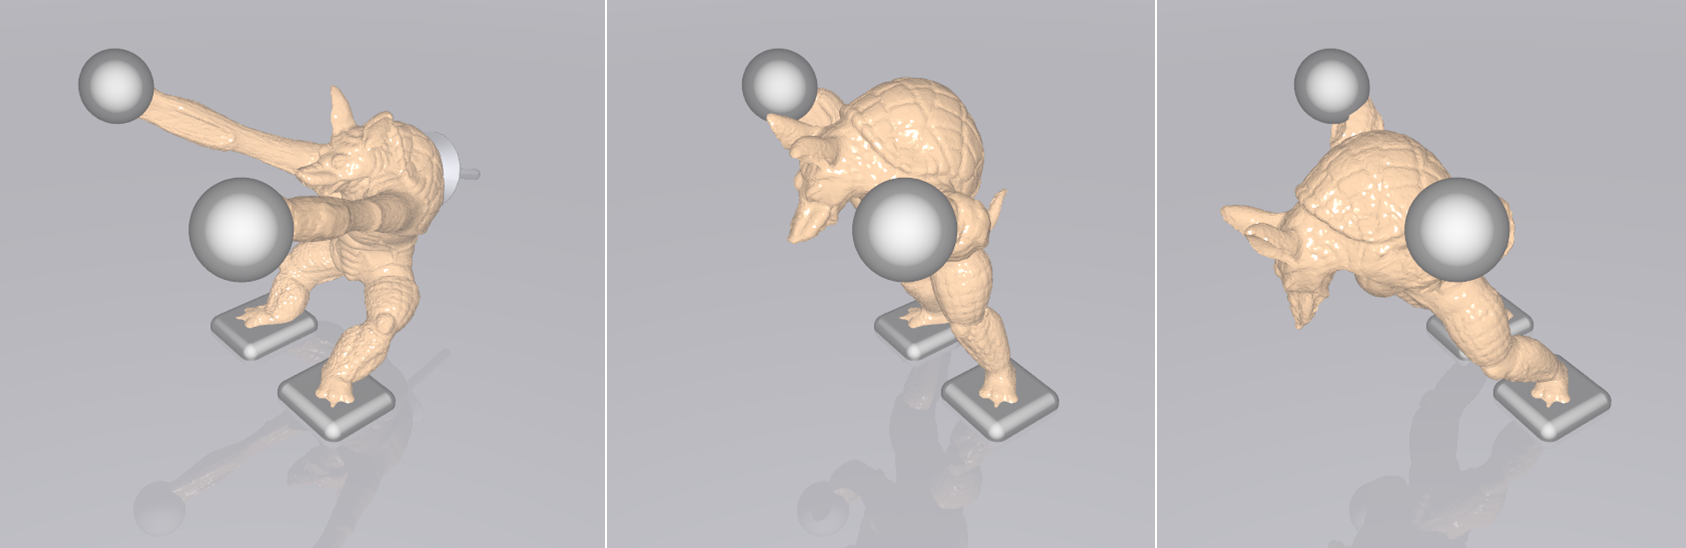
\includegraphics[width=\linewidth]{../figs/demo_pull_armadillo.png}
  \caption{\label{fig:3}
  An armadillo is initially anchored on its back and four limbs, and it deforms elastically when its back is released.
}
\end{figure}

\subsection{Plasticity}

\begin{figure}[t]
  \centering
  %\mbox{} \hfill
  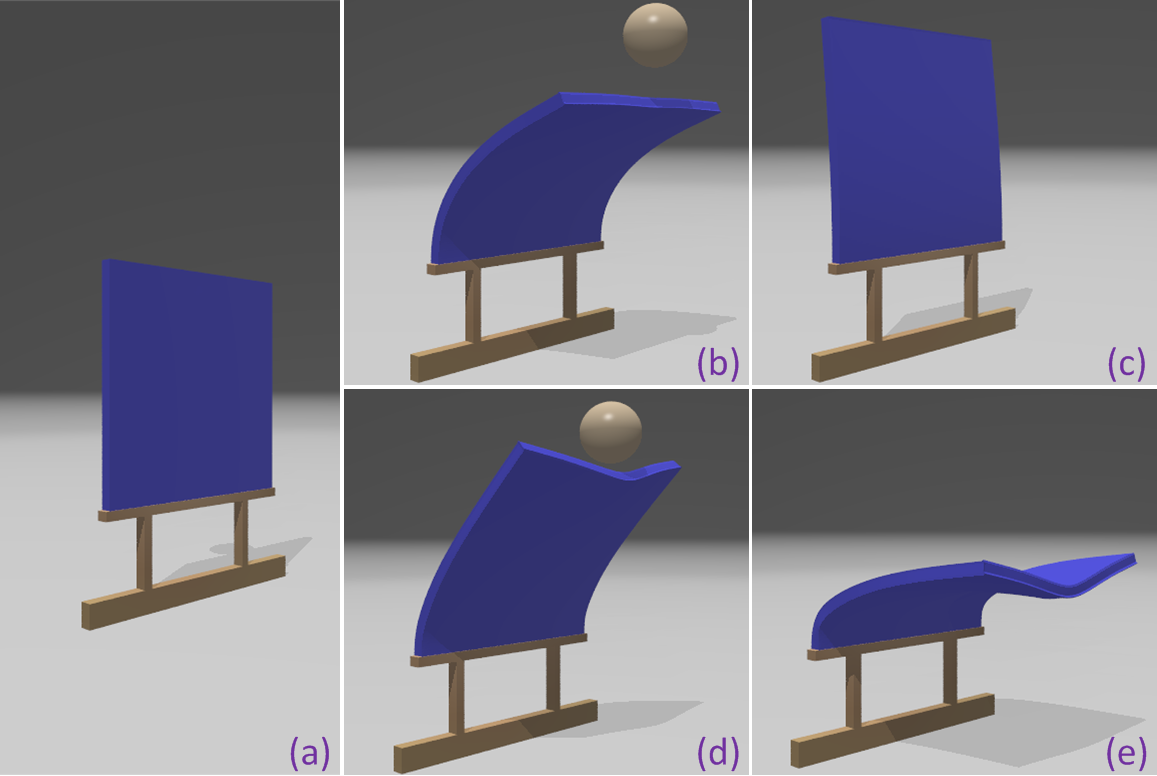
\includegraphics[width=\linewidth]{../figs/demo_impact_upside.png}
  \caption{\label{fig:4}
  Comparison of elastic and plastic deformations by shooting a sphere at two walls made of different materials with identical initial configuration as in (a). The elastic wall deforms on impact (b), and recovers afterwards (c). The plastic wall undergos permanent deformation (e) after the impact (d).
}
\end{figure}
Plasticity model for peridynamics is less studied in literature due to its complexity. To our knowledge, Silling et al. \cite{silling2007peridynamic} proposed the first plasticity model that is analogous to the von Mises flow model in classical theory. Mitchell presented a new framework for peridynamics-based plasticity modeling\cite{mitchell2011nonlocal} based on Silling et al.'s model, whereas the model hasn't been verified by experiments thus far. We adopt Mitchell's model for practical applications, and propose novel modifications based on their work.

Our plasticity model is based on purely deviatoric plastic flow theory, therefore we start by decomposing the deviatoric bond extension $e_{ij}^d$ (see Equation~\ref{eq:8}) into two components by addition:
\begin{equation}
e_{ij}^d = e_{ij}^e+e_{ij}^p,
\label{eq:10}
\end{equation}
where $e_{ij}^e$ and $e_{ij}^p$ are the elastic and plastic part of the total deviatoric bond extension respectively. To incorporate plasticity into the constitutive model,  the deviatoric part of internal force density (see Equation~\ref{eq:7}) is now redefined as below:
\begin{equation}
A_{dev} = 4\omega_{ij}b(e_{ij}^d-e_{ij}^p),
\label{eq:11}
\end{equation}
with the contribution of plastic deviatoric bond extension removed from force computation. In case of elastic deformations, the term $e_{ij}^p$ vanishes and Equation~\ref{eq:11} conforms to Equation~\ref{eq:7}.

A simple yield function $f(A_{dev})$ is used to determine whether deformation has entered the plasticity regime:
\begin{equation}
f(A_{dev}) = \frac{(A_{dev})^2}{2}-\Psi_0,
\label{eq:12}
\end{equation}
where $\Psi_0$ is a critical parameter. The deformation is elastic if $f(A_{dev})\leq 0$, and plasticity is present if  $f(A_{dev}) > 0$.

In case of plastic deformations, we project $A_{dev}$ onto the yield surface to obtain a critical value of deviatoric force density $A_{dev}^c$:
\begin{equation}
A_{dev}^c=\sqrt{2\Psi_0}\mathrm{sign}(A_{dev}),
\label{eq:13}
\end{equation}
where $\mathrm{sign}(\cdot)$ is the sign function. $A_{dev}^c$ is used to compute the increment of plastic deviatoric bond extension:
\begin{equation}
\triangle e_n^p = \frac{1}{2b}(A_{dev}-A_{dev}^c)
\label{eq:14}
\end{equation}
\begin{equation}
e_{n+1}^p = (e_n^p+\triangle e_n^p)\mathrm{min}\big(1,\frac{\gamma}{|e_n^p+\triangle e_n^p|}\big).
\label{eq:15}
\end{equation}
The subscripts $n$ and $n+1$ denote the discretized point of time at which the bond extensions and corresponding increments are evaluated. The parameter $\gamma$ which does not appear in the original model of Mitchell's \cite{mitchell2011nonlocal} is used to enforce a limit on the amount of plasticity. We found in experiments that with this parameter we obtain more control over the plastic behaviors (see Figure~\ref{fig:5}) and the stability of simulation is improved as well. Figure~\ref{fig:4} shows a comparison of the simulation results using our elastoplastic constitutive model. Our elastic model produces correct elastic behaviors, and permanent deformation is captured when plasticity is involved.
\subsection{Anisotropy}

Our constitutive model is isotropic up to now, and we extend it to anisotropy in this section. We model anisotropy by manipulating the weight functions between particles (see Equation~\ref{eq:4}) with direction information. The key idea is to associate an anisotropy matrix $\mathbf{G}$ with each particle, so that applying the transformation to the bond between particles biases the influence weight toward preferred directions. The weight function $\omega_{ij}$ for anisotropic materials is computed as below:
\begin{equation}
\omega_{ij}=\frac{\delta}{|\mathbf{G}(\mathbf{x}_j-\mathbf{x}_i)|}.
\label{eq:16}
\end{equation}
Appealing anisotropic effects could be generated with our anisotropy model. See Figure~\ref{fig:1} for a demonstration of the model applied to brittle and ductile fracture animation. Figure~\ref{fig:6} compares the crack patterns generated by the brittle fracture examples in Figure~\ref{fig:1}.

\begin{figure}[t]
  \centering
  %\mbox{} \hfill
  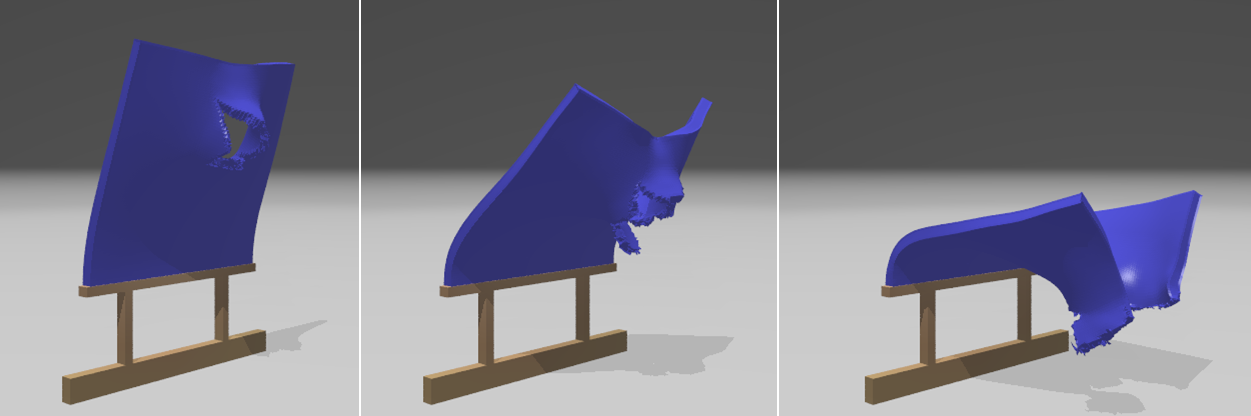
\includegraphics[width=\linewidth]{../figs/demo_impact_upside_plastic_fracture.png}
  \caption{\label{fig:5}
  Simulation of ductile fracture with different amount of maximum plasticity. From left to right the parameter $\frac{\gamma}{|\mathbf{x}_j-\mathbf{x}_i|}$ is 0.1,0.15, and 0.2.
}
\end{figure}
\begin{figure}[t]
  \centering
  %\mbox{} \hfill
  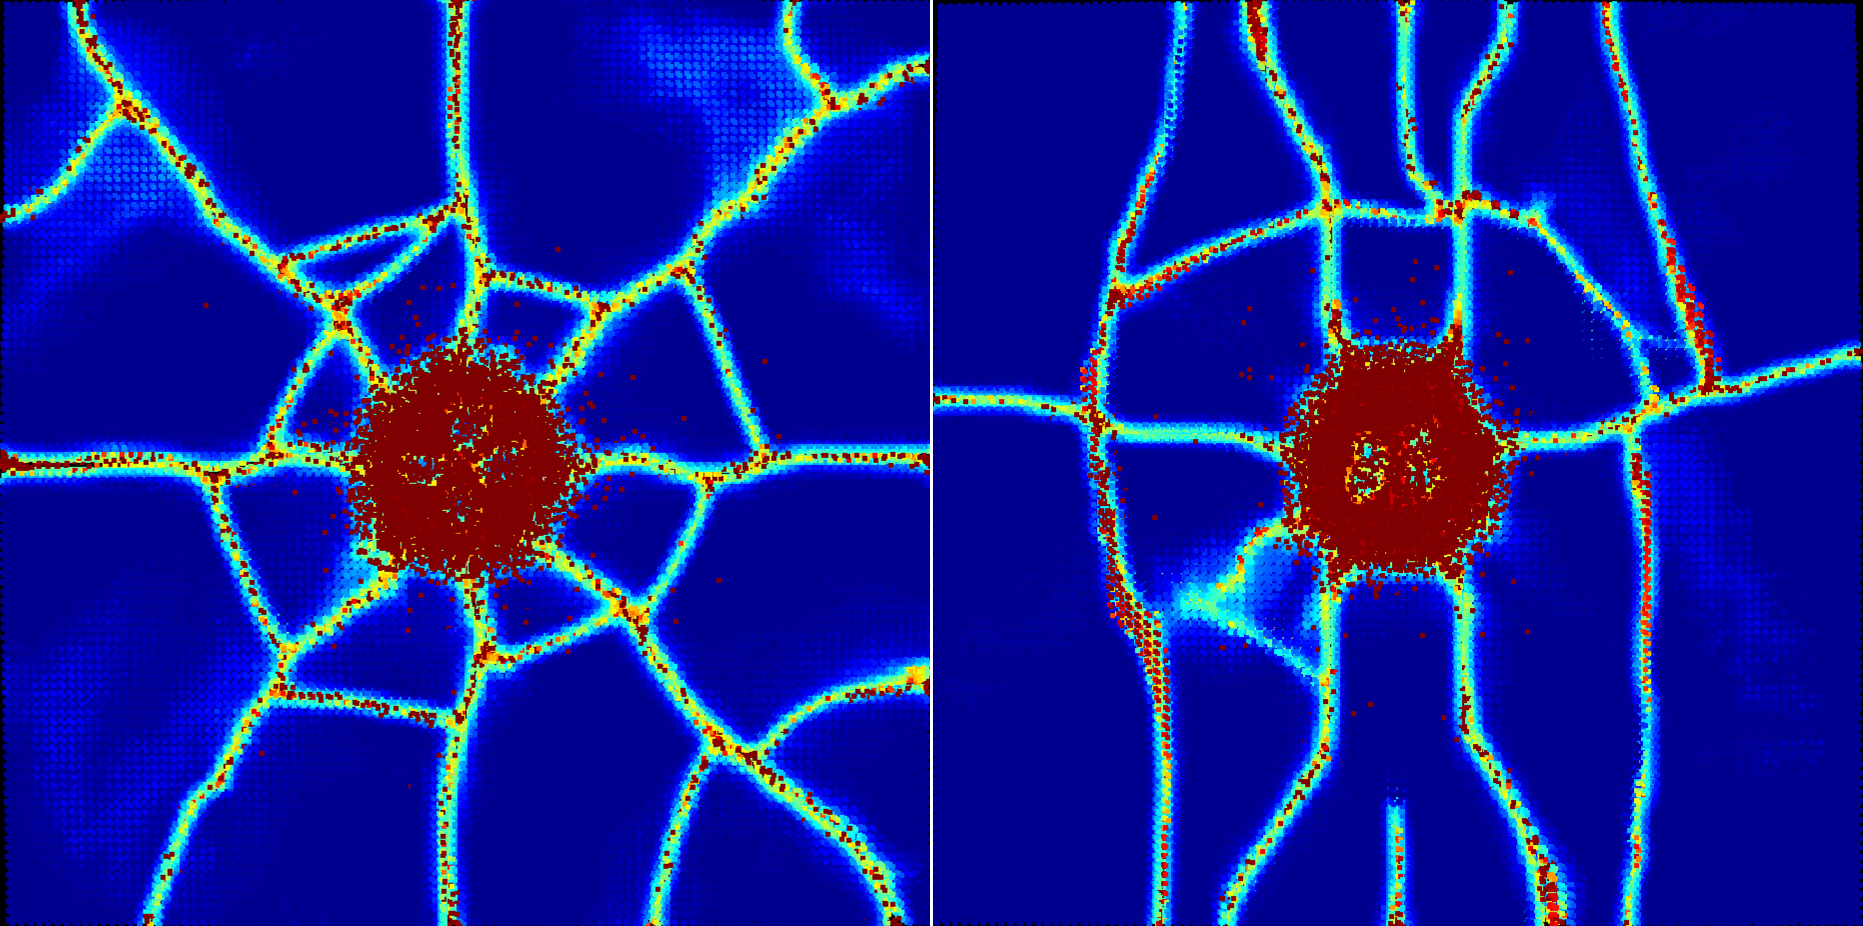
\includegraphics[width=\linewidth, bb=0 0 1400 700]{../figs/demo_impact_color_map.png}
  \caption{\label{fig:6}
  Comparison of crack patterns generated by isotropic (left) and anisotropic (right) brittle fracture. The color represents the damage of particles, with blue as no damage and red as complete damage.
}
\end{figure}
%-------------------------------------------------------------------------
\section{Fracture}

In this section we present our fracture model and introduce the mesh embedding strategy we employ to generate crack surfaces.

\subsection{Fracture Criterion}

Material damage can be modeled in peridynamics by permanently eliminating the bonds between particles. The dynamics with discontinuities is trivial due to the integral-based nature of peridynamics. For elastic brittle materials, a simple critical stretch is generally used as the fracture criterion. This criterion conforms to the physically plausible energy release rate, and it has been validated before \cite{Silling2005}. Levine et al.\cite{Levine:2015:PPS:2849517.2849526} also utilized this criterion for brittle fracture modeling in computer graphics. In order to account for plasticity and model ductile fracture, we redefined the elastic critical stretch criterion as:
\begin{equation}
s_{ij}^e =\frac{e_{ij}-e_{ij}^p}{|\mathbf{x}_i-\mathbf{x}_j|}.
\label{eq:17}
\end{equation}

Unfortunately, we found in experiments that this fracture criterion would cause unrealistic artifacts since bonds with smaller rest lengths are sometimes more prone to breaking. We alleviate this problem by incorporating the weight function $\omega_{ij}$ into the criterion to increase the fracture criterion of closer family members. Shattering effects could arise for brittle materials, which lead to many tiny fragments. We could avoid the generation of too small fragments by continuously increasing the crack threshold as the material gets damaged. The final fracture criterion that we employ in our model is formulated as below:
\begin{equation}
s_{ij}^\omega = (1 + \alpha\phi)\frac{s_{ij}^e}{\omega_{ij}} = (1 + \alpha\phi)\frac{e_{ij}-e_{ij}^p}{\delta},
\label{eq:18}
\end{equation}
where $\phi = 1 - \frac{n_i}{N_i}$ measures the damage level of material point $i$. $n_i$ and $N_i$ are the numbers of active bonds connecting $i$ with its family members in the deformed and initial configurations, respectively. $n_i$ gradually decreases as more bonds around $i$ are broken, increasing the damage level of $i$. The parameter $\alpha$ is set to 0 by default, and could be used to mitigate the shattering effect while non-zero values are given.
Figure~\ref{fig:7_after} provides an example of controlling the dust with different $\alpha$ values.
It shows that our criterion is able to produce compelling results in practical use.

\begin{figure}[t]
  \centering
  %\mbox{} \hfill
  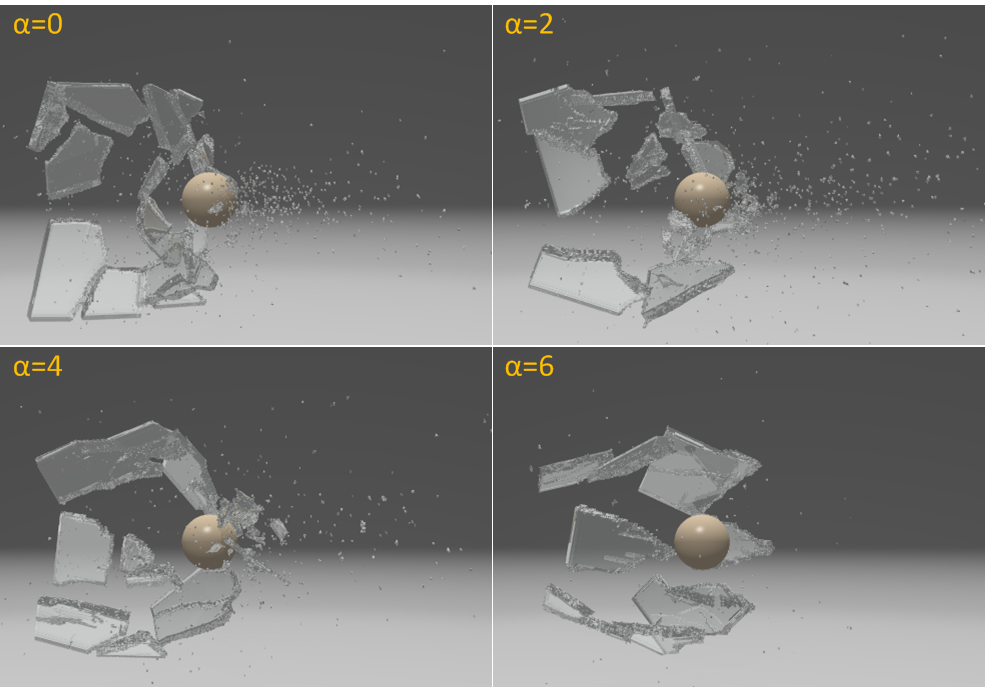
\includegraphics[width=\linewidth]{../figs/revision/demo_shatter_control.png}
  \caption{\label{fig:7_after}
  Glass wall fracture with different $\alpha$ values.
}
\end{figure}
\subsection{Embedded Mesh}
%While our point-based geometry representation offers great simplicity, this simplicity does come at a cost that it is difficult to generate render geometry. To model realistic fracture, sharp edges are required on the crack surfaces. This naturally motivates us to embed a volumetric mesh into our system.
%Given a tetrahedron mesh, we first initialize our particles to the center of elements and its family members through a pre-specified horizon $\delta$.
%Each particle that represents a single tetrahedron has a common face shared for each immediate neighbor.
%%Previous methods such as \cite{Chen2013} usually utilize a face-copying strategy to reflect fracture within a meshless framework.
%%However, this is only practical for brittle material where two copied crack triangle faces are either coincident or completely separated.
%%In our method, we turn face-copying into a vertex-splitting strategy similar to the FEM to enable us adjust the topology for deformation objects.
%To accommodate the topology changes resulted from fracture, we propose a simple strategy that dynamically split the embedded mesh along the elements.
%Our method takes the sprits from \cite{Chen2013} but improves their idea to model fracture for deformable objects.
%In their method, faces are copied if fracture occur between two neighboring elements.
%However, it becomes impracticable for deformable objects since we can't decide which copied vertex to replace the origin vertex,
%although it is not a question in brittle material as these two faces are either completely coincident or separated.
%
%The key to overcome this problem is our temporarily postponing the splitting until other crack faces are added to be able to result in a vertex-splitting .
%For fracture occurring between two immediate particles, the shared triangle is marked and added to a crack face set.
%We can merely investigate those vertices that involved in crack face set at each time step since only these vertices have the ability to split.
%For each crack vertex, we determine whether its connected tetrahedra have been separated by crack faces.
%If this is the case, we split the vertex, assign corresponding tetrahedra to each of them, and make a topological change on the embedded mesh.
%After that, we could safely remove those crack faces that directly results in our vertex splitting.
%If the connected tetrahedra are separated into more than two groups, we also split vertex into multiple copies accordingly.
%Moveover, simultaneous splitting of multiple vertices at one crack edge are also compatible in our method.
%Our method is simply yet efficient.
%But one drawback is that it require a relatively high resolution and reasonable discretization of mesh to avoid the jaggy artifact.
%Figure~\ref{fig:6} shows an example of using our strategy to produce complex crack surfaces.

%After handling fractures, we finally update the vertex position with respect to the current velocities of its connected particles.
%We simply employ a weighted average approach to move our vertices, which is
%\begin{eqnarray}
%W_{\mathrm{v}} &=& \sum_{\mathrm{p}} \frac{1}{4}m_{\mathrm{p}}\\
%\textbf{v}_{\mathrm{v}} &=& \frac{1}{W_{\mathrm{v}}}\sum_{\mathrm{p}}\frac{1}{4}m_{\mathrm{p}}\textbf{v}_{\mathrm{p}}\\
%\mathrm{new\_pos} &\leftarrow& \mathrm{old\_pos} + \Delta t\textbf{v}_{\mathrm{v}}
%\end{eqnarray}
%where subscripts $\mathrm{p}$ and $\mathrm{v}$ represent particle and vertex, respectively.
%$m_{\mathrm{p}}$ is the mass of the particle, $\textbf{v}_{\mathrm{v}}$ and $\textbf{v}_{\mathrm{p}}$ denote the velocity.
%For rendering, a surface mesh is extracted from the volumetric mesh at the end of each frame.

While particle-based discretization offers great simplicity, this simplicity does come at a cost that it is difficult to generate surface representation. This naturally motivates the use of mesh embedding approach, in which the boundary of volumetric meshes could represent the original object surface and the newly generated crack surfaces during simulation. We use tetrahedron meshes to represent object geometry, and the particles are initialized at the barycenters of each mesh element.
The particle family members are initialized according to the mesh connectivity and a pre-specified horizon $\delta$.
To accommodate the topology changes resulted from fracture, we propose a simple strategy that dynamically split the embedded mesh along the elements.

We achieve this by maintaining a crack face set and continuously adding the shared triangles to it for fracture happened between immediate elements.
At each time step, we investigate merely those vertices that involved in crack face set and determine whether its connected tetrahedra have been separated by crack faces.
If this is the case, we split the vertex, assign corresponding tetrahedra to each of them, and make a topological change on the embedded mesh.
After spliting, we could safely remove only those crack faces that directly results in our vertex splitting.
If the connected tetrahedra are separated into more than two groups, we accordingly split vertex into multiple copies.
Simultaneous splitting of multiple vertices at one crack face are also compatible in our method.
Figure~\ref{fig:7} shows an example of using our strategy to produce complex crack surfaces.

After handling mesh topology, we update the vertex positions using the velocities of corresponding particles.
A simple weighted-average approach is employed to update the vertex positions:
\begin{eqnarray}
\omega_{\mathrm{v}} &=& \sum_{\mathrm{p}} \frac{1}{4}m_{\mathrm{p}}\\
\textbf{v}_{\mathrm{v}} &=& \frac{1}{\omega_{\mathrm{v}}}\sum_{\mathrm{p}}\frac{1}{4}m_{\mathrm{p}}\textbf{v}_{\mathrm{p}}\\
\mathbf{x}_{\mathrm{v}}^{t+1} &=& \mathbf{x}_{\mathrm{v}}^{t} + \Delta t\textbf{v}_{\mathrm{v}}
\end{eqnarray}
where subscripts $\mathrm{p}$ and $\mathrm{v}$ represent the particle and the mesh vertex respectively.
$m_{\mathrm{p}}$ and $\textbf{v}_{\mathrm{p}}$ are the mass and velocity of the particle, $\textbf{v}_{\mathrm{v}}$ and $\textbf{x}_{\mathrm{v}}$ are the velocity and position of the mesh vertex.

\begin{figure}[t]
  \centering
  %\mbox{} \hfill
  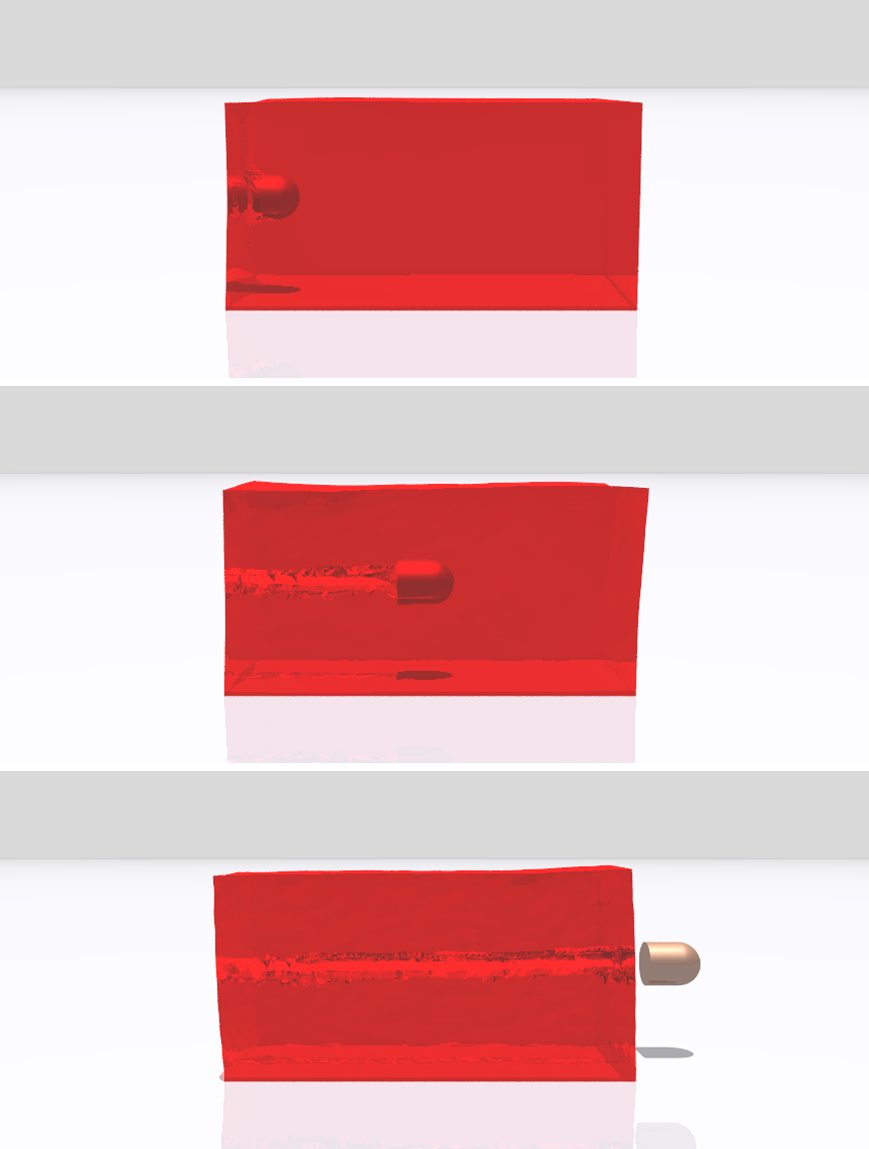
\includegraphics[width=\linewidth]{../figs/demo_jello.png}
  \caption{\label{fig:7}
  Shooting a bullet through a jello, producing complex crack surfaces.
}
\end{figure}
\begin{figure}[t]
  \centering
  %\mbox{} \hfill
  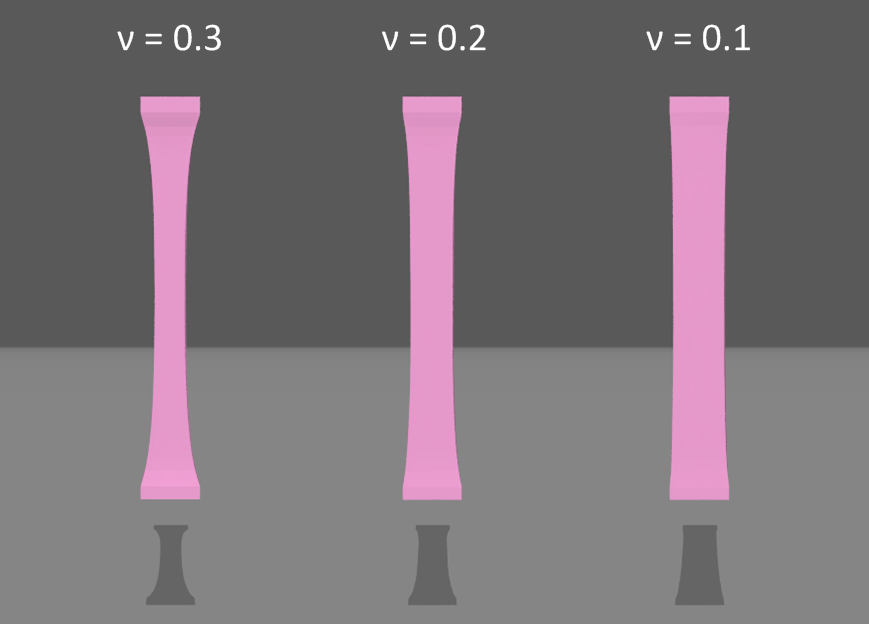
\includegraphics[width=\linewidth]{../figs/compare_different_poisson_ratio.png}
  \caption{\label{fig:8}
  Simulation of stretching beams with different Poisson ratios.
}
\end{figure}
%-------------------------------------------------------------------------
\section{Results}

We present the results produced with our method in this section. All our examples are run on a 3.5GHz, Intel Core i7-5930K CPU with 32G RAM. The embedded tetrahedron meshes are generated using the open-source TetGen software \cite{Si:2015:TDQ:2732672.2629697}. All the figures in the paper are rendered off-line using the open-source POV-Ray software (\url{http://www.povray.org/}). We use explicit time integration for ease of implementation. We also performed a naive parallelized implementation of our method using OpenMP.

\noindent{\textbf{Constitutive model validation.}} We validate our constitutive model by simulating deformations with varied material properties and performing comparisons with the results of FEM. Figure~\ref{fig:3} shows an example of isotropic elastic deformations, where the back and four limbs of an armadillo are initially anchored and then the anchor on the back is removed. The deformations are plausible and no undesirable numerical fracture occurs when the arms of the armadillo are over-stretched. In Figure~\ref{fig:4} we compare the results of elasticity and plasticity, and our model produces correct deformation behaviors. Figure~\ref{fig:5} demonstrates the varied effects produced by tunning the amount of maximum plasticity. Figure~\ref{fig:8} compares the elastic deformations of stretching beams with different Poisson ratio values. Unlike Levine et al.'s model \cite{Levine:2015:PPS:2849517.2849526}, our constitutive model is not limited to a single Poisson ratio. Finally, we conduct comparisons with FEM through Figure~\ref{fig:9} to Figure~\ref{fig:12}.
The deformations of a bending beam in Figure~\ref{fig:9} produced with our method are almost identical to those generated by FEM, under both stiff and soft material settings. We further demonstrate the accuracy of our method in constitutive modeling using comparisons with quantitative error analysis. The swing (see Figure~\ref{fig:10}) and twist (see Figure~\ref{fig:11}) deformations of the bar produced by our method are as accurate as those by corotated linear FEM with position deviations less than $10\%$. The position deviations are measured over the diagonal of the object's bounding box: $Error = \frac{|\bm{x}_p-\bm{x}_p^{ref}|}{d}$ where $d$ is the length of the diagonal. Note that our constitutive model alleviates artifacts of the classical linear model albeit derived from it. It is because peridynamics does not employ the geometric linear approximation as the Cauchy strain in continuum mechanics does. Thus peridynamics does not suffer from ghost forces while undergoing rigid rotations, even though the constitutive relation is linear. We also obtain nice accuracy for the noncyclic vibrations of the armadillo presented in Figure~\ref{fig:12}. Therefore, we believe our peridynamics-based constitutive model is plausible for graphical animations.

\begin{figure}[t]
  \centering
  %\mbox{} \hfill
  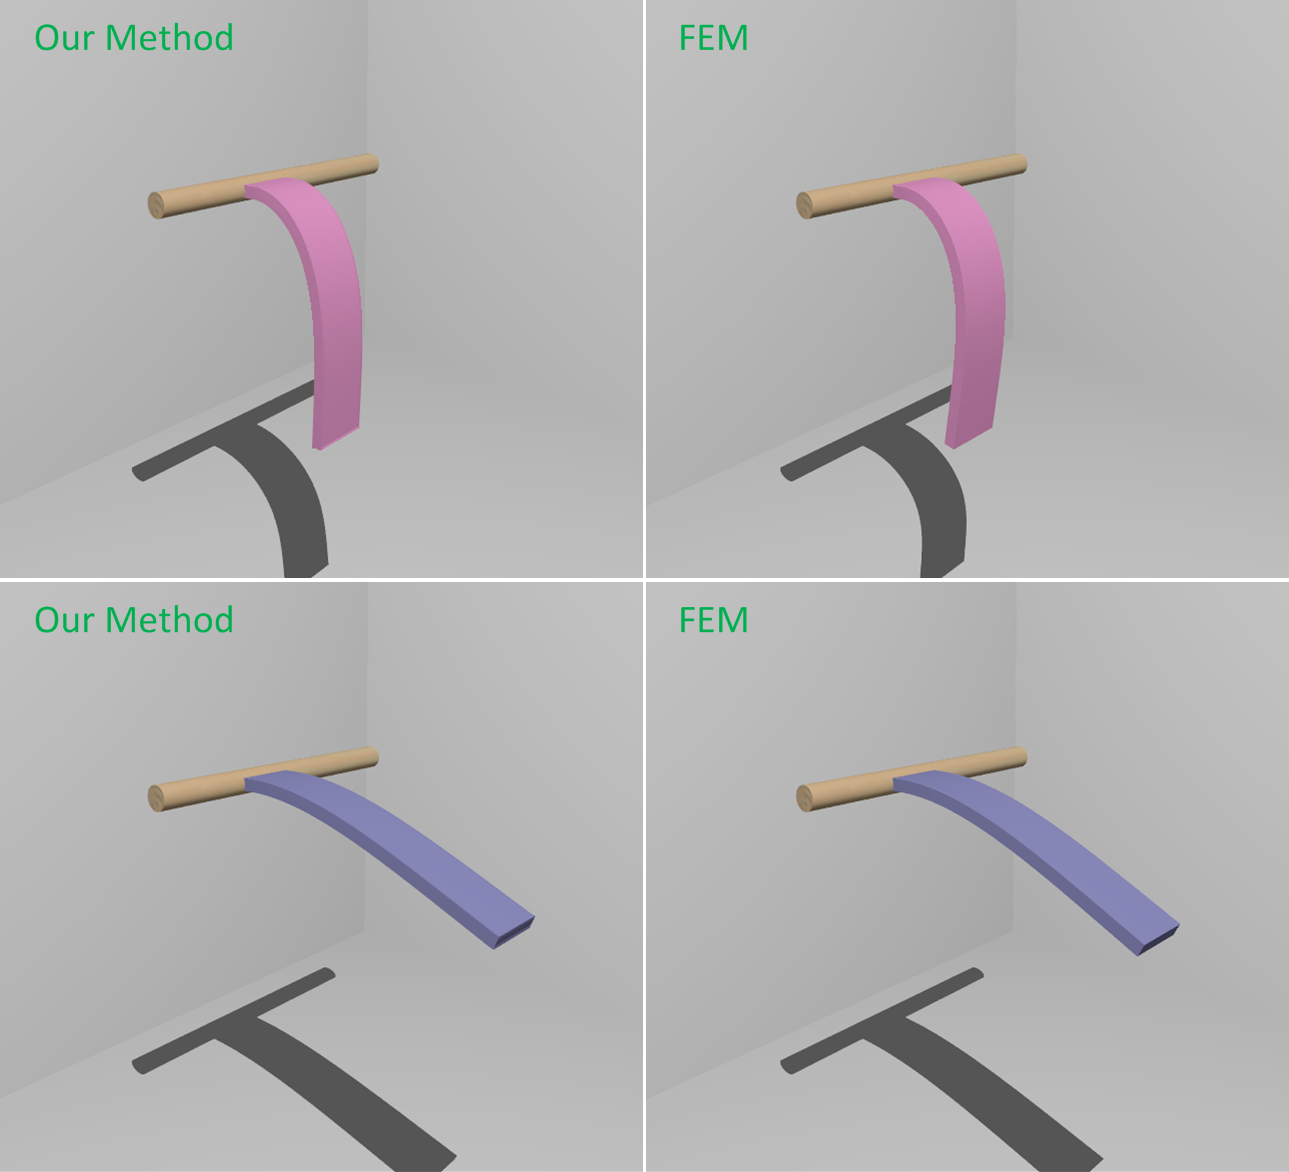
\includegraphics[width=\linewidth]{../figs/demo_strip_vs_fem.png}
  \caption{\label{fig:9}
  Simulation of bending beams with different stiffness (top:soft;bottom:stiff) using our method and FEM. The results of our method are indistinguishable from the results produced by FEM.
}
\end{figure}
\begin{figure}[t]
  \centering
  %\mbox{} \hfill
  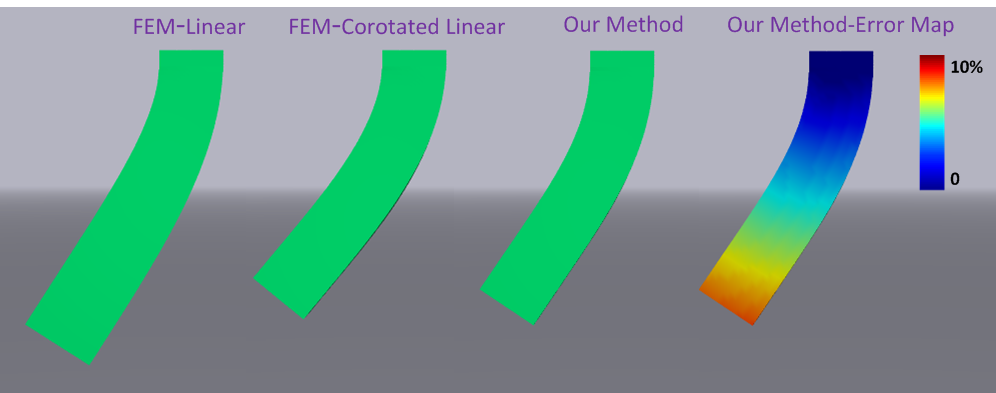
\includegraphics[width=\linewidth]{../figs/revision/demo_bar_oscillate_vs_fem_2.png}
  \caption{\label{fig:10}
  Simulation of a swinging bar using linear FEM (left), corotated linear FEM (middle left), and our method (middle right). Our method is accurate as the corotated linear FEM (right).
}
\end{figure}
\begin{figure}[t]
  \centering
  %\mbox{} \hfill
  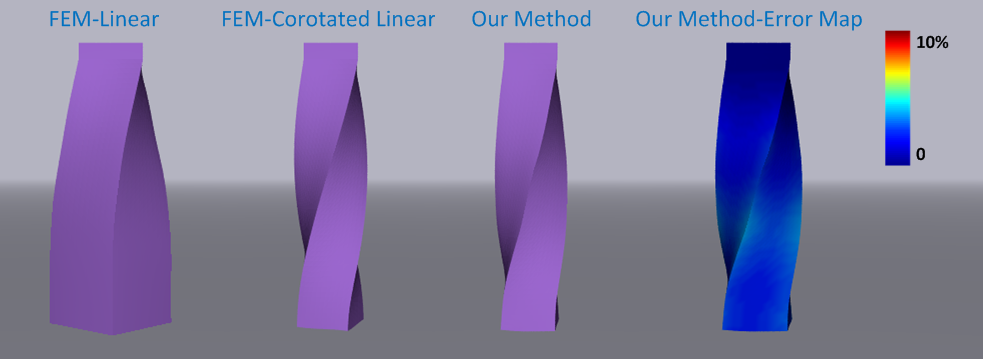
\includegraphics[width=\linewidth]{../figs/revision/demo_bar_twist_vs_fem.png}
  \caption{\label{fig:11}
  Simulation of a twisting bar using linear FEM (left), corotated linear FEM (middle left), and our method (middle right). Our method is accurate as the corotated linear FEM (right).
}
\end{figure}
\begin{figure}[t]
  \centering
  %\mbox{} \hfill
  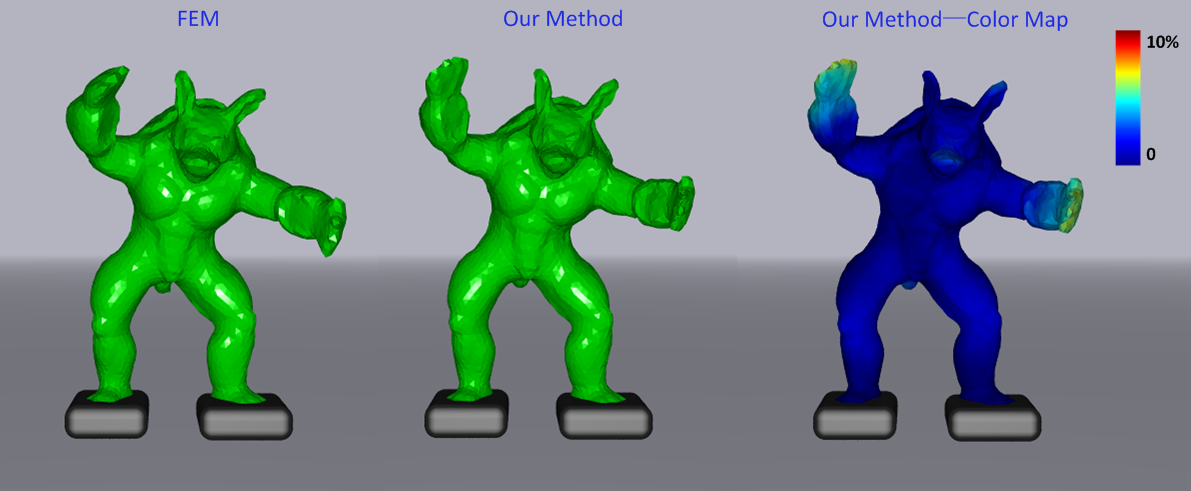
\includegraphics[width=\linewidth]{../figs/revision/demo_armadillo_vs_fem_2.png}
  \caption{\label{fig:12}
  Simulation of noncyclic vibrations for an armadillo using FEM (left) and our method (middle). The accuracy of our method is acceptable compared with FEM (right).
}
\end{figure}

\noindent{\textbf{Fracture animation.}} Our method could simulate brittle and ductile fracture with compelling visual realism. In Figure~\ref{fig:1} a wide range of fracture behaviors are generated, including isotropic brittle fracture, anisotropic brittle fracture, isotropic ductile fracture, and anisotropic ductile fracture. This demonstrates the capability of our method in simulating fracture. We believe our approach is the first peridynamics-based framework in graphics with such flexibility. Figure~\ref{fig:7} shows an example of shooting a bullet into a jello-like object. Our method handles well the generation of the complex crack surfaces. The armadillo in Figure~\ref{fig:13} is stretched until its limbs tear off. The behavior of ductile fracture is correctly demonstrated, including the progressive generation of multiple cracks (see Figure~\ref{fig:17}). The glass wall in Figure~\ref{fig:14} is pressed by a heavy metal ball. Cracks develop and propagate without shattering the glass into fragments. This phenomenon cannot be reproduced by the level set approach \cite{Hegemann:2013:LSM:2485895.2485908} as mentioned in their paper, and it is challenging for the remeshing-based FEM methods \cite{O'Brien:1999:GMA:311535.311550,O'Brien:2002:GMA:566654.566579} considering the mesh operations. In contrast, our method handles the complicated propagation process well, including the branching and merging of cracks. In Figure~\ref{fig:15} a bunny made of elastic material falls to the ground and shatters. Our method is able to realistically capture the secondary fracture of the fragments. Figure~\ref{fig:16} is another demonstration of our method in handling crack tips. A thin sheet with initial cracks is torn on two sides. The cracks gradually proceed and finally shatter the sheet. Please note the filaments generated as a result of crack branching and merging.

In Table~\ref{tab:1} we list the detailed parameter settings and the performance data for all the examples presented in the paper. The results in this paper are produced with practical computation time.
\begin{table*}[htb]
\resizebox{\textwidth}{!}{
\begin{tabular}{lccccccccccc}
  \hline
  \hline
  Examples & particle num & $\delta$ & bond num & $\kappa$ & $\mu$ & $\rho$            & $\Psi_0$ & $\frac{\gamma}{|\mathbf{x}_j-\mathbf{x}_i|}$ & $s^w_{(k)(j)}$ & $\Delta t$ & performance\\
           &              &          &          &   (KPa)   & (KPa)  &(Kg/$\mathrm{m}^3)$&          &                                              &                & (s)       &(s/step)\\
  \hline
  Glass Wall[Figure~\ref{fig:1}(a)(b), Figure ~\ref{fig:7_after},~\ref{fig:14}]     & $3.0\times10^5$ & 1.45$\lambda$ & $5.0\times10^7$ & $3.3\times10^{7}$ & $2.0\times10^{7}$        & 2200 & $\infty $ & 0.0             & 0.0005   & $1.0\times10^{-6}$          & $\sim2.4$ \\
  Plastic Wall [Figure~\ref{fig:1}(c)(d)]  & $3.0\times10^5$ & 1.45$\lambda$ & $5.0\times10^7$ & $3.3\times10^{3}$ & $2.0\times10^{3}$        & 2200 & $10^{25}$ & 0.2             & 0.05     & $1.0\times10^{-4}$          & $\sim2.4$ \\
  Armadillo [Figure~\ref{fig:3}]           & $4.2\times10^5$ & 1.50$\lambda$ & $7.5\times10^7$ & $6.3\times10^4$   & $3.8\times10^4$          & 1000 & $\infty $ & 0.0             & $\infty$ & $1.0\times10^{-4}$          & $\sim5.3$ \\
  Elastic Wall [Figure~\ref{fig:4}(b)(c)]  & $3.0\times10^5$ & 1.45$\lambda$ & $5.0\times10^7$ & $1.0\times10^{4}$ & $6.0\times10^{3}$        & 1200 & $\infty $ & 0.0             &$\infty$  & $5.0\times10^{-5}$   & $\sim2.4$ \\
  Plastic Wall [Figure~\ref{fig:4}(d)(e)]  & $3.0\times10^5$ & 1.45$\lambda$ & $5.0\times10^7$ & $1.0\times10^{4}$ & $6.0\times10^{3}$        & 1200 & $10^{26}$ & 0.2             & $\infty$ & $5.0\times10^{-5}$   & $\sim2.4$ \\
  Wall [Figure~\ref{fig:5}]                & $3.0\times10^5$ & 1.45$\lambda$ & $5.0\times10^7$ & $1.0\times10^{4}$ & $6.0\times10^{3}$        & 1200 & $10^{26}$ &$(0.1,0.15,0.2)$ &$\infty$  & $5.0\times10^{-5}$   & $\sim2.4$ \\
  Jello [Figure~\ref{fig:7}]               & $4.6\times10^5$ & 1.45$\lambda$ & $8.6\times10^7$ & $1.0\times10^3$   & $4.6\times10^2$          & 1000 & $\infty $ & 0.0             & 0.4      & $5.0\times10^{-5}$   & $\sim3.8$ \\
  Beam Stretch [Figure~\ref{fig:8}]        & $2.2\times10^4$ & 1.0 $\lambda$ & $1.3\times10^6$ & $2.0\times10^3$   & $(9.2,1.5,2.2)\times10^2$& 1000 & $\infty$  & 0.0             &$\infty$  & $1.0\times10^{-5}$ & $\sim0.2$ \\
  Soft Beam Bend [Figure~\ref{fig:9}]      & $4.5\times10^4$ & 1.0 $\lambda$ & $6.9\times10^6$ & $6.3\times10^3$   & $3.8\times10^3$          & 1000 & $\infty $ & 0.0             & $\infty$ & $5.0\times10^{-5}$   & $\sim0.6$ \\
  Stiff Beam Bend [Figure~\ref{fig:9}]     & $4.5\times10^4$ & 1.0 $\lambda$ & $6.9\times10^6$ & $3.3\times10^4$   & $2.0\times10^4$          & 1000 & $\infty $ & 0.0             & $\infty$ & $2.5\times10^{-5}$ & $\sim0.6$ \\
  Bar Swing [Figure~\ref{fig:10}]     & $9.2\times10^3$ & 1.11 $\lambda$ & $1.5\times10^5$ & $5.0\times10^3$   & $5.0\times10^3$          & 1000 & $\infty $ & 0.0             & $\infty$ & $1.0\times10^{-4}$ & $\sim0.05$ \\
  Bar Twist [Figure~\ref{fig:11}]     & $9.2\times10^3$ & 1.34 $\lambda$ & $1.5\times10^5$ & $1.0\times10^3$   & $6.0\times10^2$          & 1000 & $\infty $ & 0.0             & $\infty$ & $1.0\times10^{-4}$ & $\sim0.06$ \\
  Armadillo Vibrate [Figure~\ref{fig:12}]     & $2.0\times10^4$ & 1.38 $\lambda$ & $1.8\times10^6$ & $5.0\times10^3$   & $3.0\times10^3$          & 1000 & $\infty $ & 0.0             & $\infty$ & $5.0\times10^{-4}$ & $\sim0.2$ \\
  Armadillo [Figure~\ref{fig:13}]          & $4.2\times10^5$ & 1.50$\lambda$ & $7.5\times10^7$ & $6.3\times10^4$   & $3.8\times10^4$          & 1000 & $\infty $ & 0.0             & 0.61     & $1.0\times10^{-4}$          & $\sim5.3$ \\
  Bunny [Figure~\ref{fig:15}]              & $5.2\times10^5$ & 1.45$\lambda$ & $8.8\times10^7$ & $2.5\times10^2$   & $1.2\times10^2$          & 1000 & $\infty $ & 0.0             & 0.13     & $5.0\times10^{-4}$          & $\sim5.2$ \\
  Thin Sheet [Figure~\ref{fig:16}]              & $1.6\times10^5$ & 1.45$\lambda$ & $2.0\times10^7$ & $5.0\times10^3$   & $3.0\times10^3$          & 1000 & $\infty $ & 0.0             & 0.1     & $5.0\times10^{-5}$          & $\sim1.8$ \\
  \hline
\end{tabular}
}
\caption{Model information, simulation parameters, and performance data for all our examples. $\lambda$ is the average edge length of the embedded tetrahedron mesh used for particle initiation.}
\label{tab:1}
\end{table*}
\begin{figure*}[t]
  \centering
  %\mbox{} \hfill
  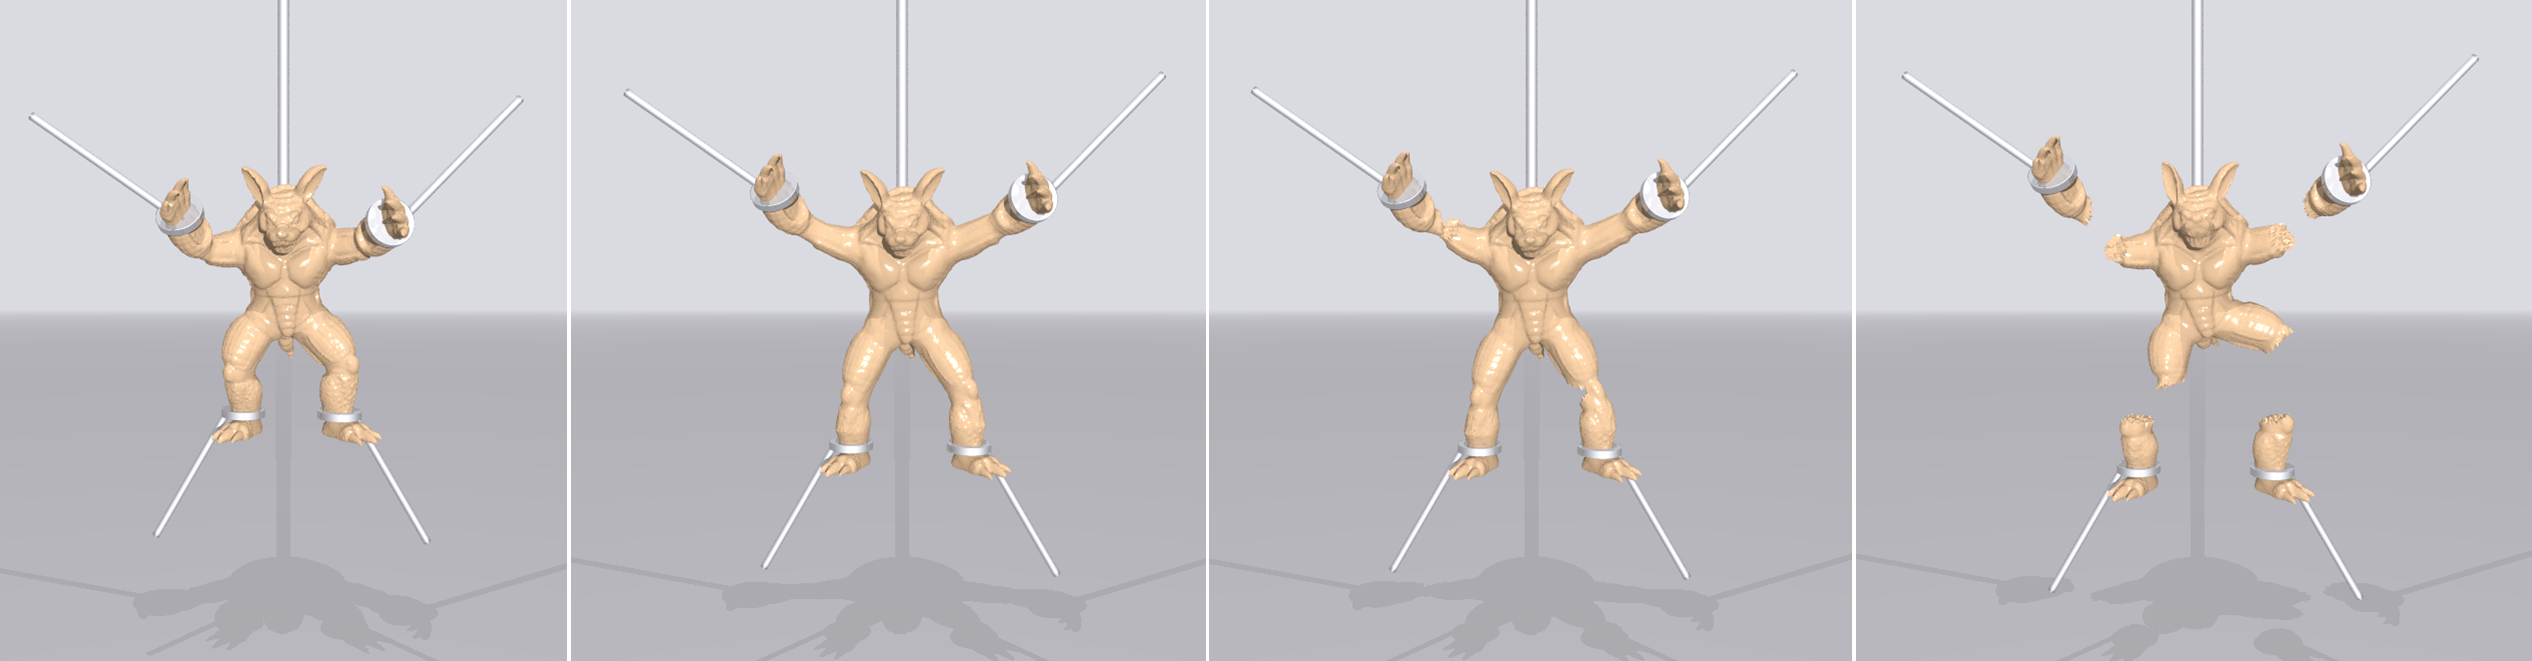
\includegraphics[width=\linewidth]{../figs/demo_tear_armadillo.png}
  \caption{\label{fig:13}
  An armadillo is stretched until its limbs tear off.
}
\end{figure*}

%-------------------------------------------------------------------------
\section{Discussions}
We have introduced a novel meshless framework for graphical modeling and animation of elastoplastic solids. Our work is the first peridynamics-based framework in computer graphics that can simulate a wide range of material behaviors, including elasticity, plasticity, and fracture.

Our work is not without limitations. Currently we can not afford large time steps because we used explicit time integration in our implementation. In the future, we plan to incorporate implicit time integration into our framework to achieve less restricted time step size. Another limitation of our work stems from the mesh embedding strategy for crack surface representation. The level of crack detail is highly dependent on the embedded mesh resolution. In addition, we generate crack surfaces by separating the mesh elements, which could cause the zig-zag artifact (see Figure~\ref{fig:17}). This artifact might be alleviated by smoothing the crack surfaces somewhat, or employing the virtual node algorithm. While we used multi-threading in our implementation, the performance of our method could be further improved with GPGPU techniques.

Other interesting avenues for future work include combining peridynamics theory with existing methods from classical theory such as FEM and SPH. These methods complement each other, and their combination could produce a new method that is more powerful for animation production.
\begin{figure*}[t]
  \centering
  %\mbox{} \hfill
  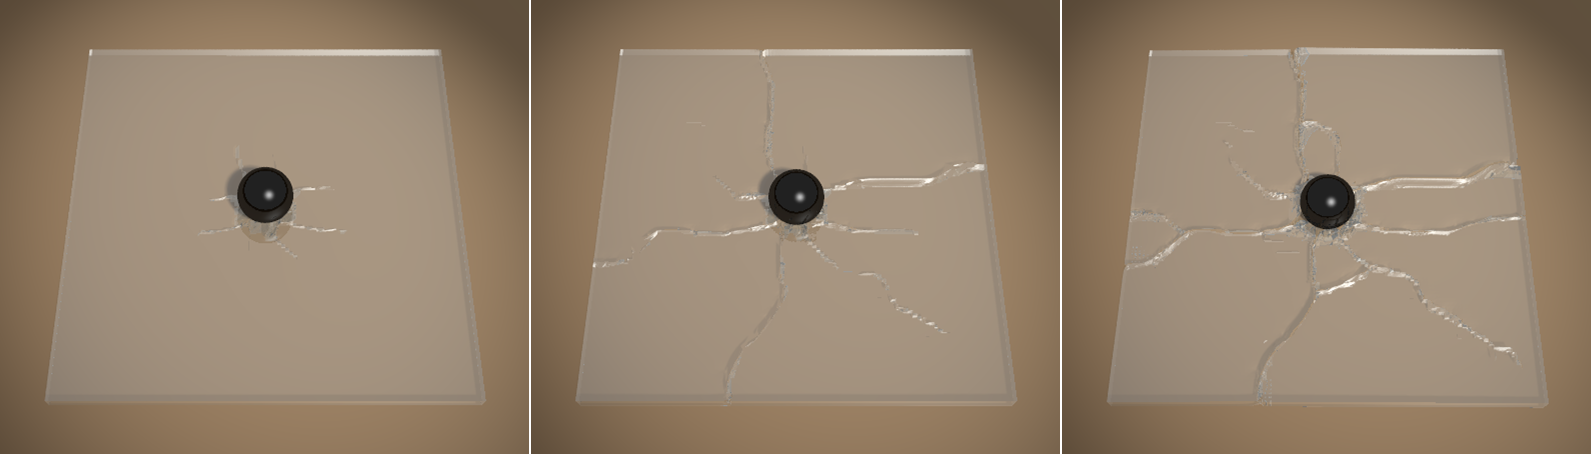
\includegraphics[width=\linewidth]{../figs/revision/demo_brittle_fall.png}
  \caption{\label{fig:14}
  A glass wall on ground is pressed by a heavy metal ball and cracks without separating. Our method can model the complicated crack propagation process, including branching and merging.
}
\end{figure*}
\begin{figure*}[t]
  \centering
  %\mbox{} \hfill
  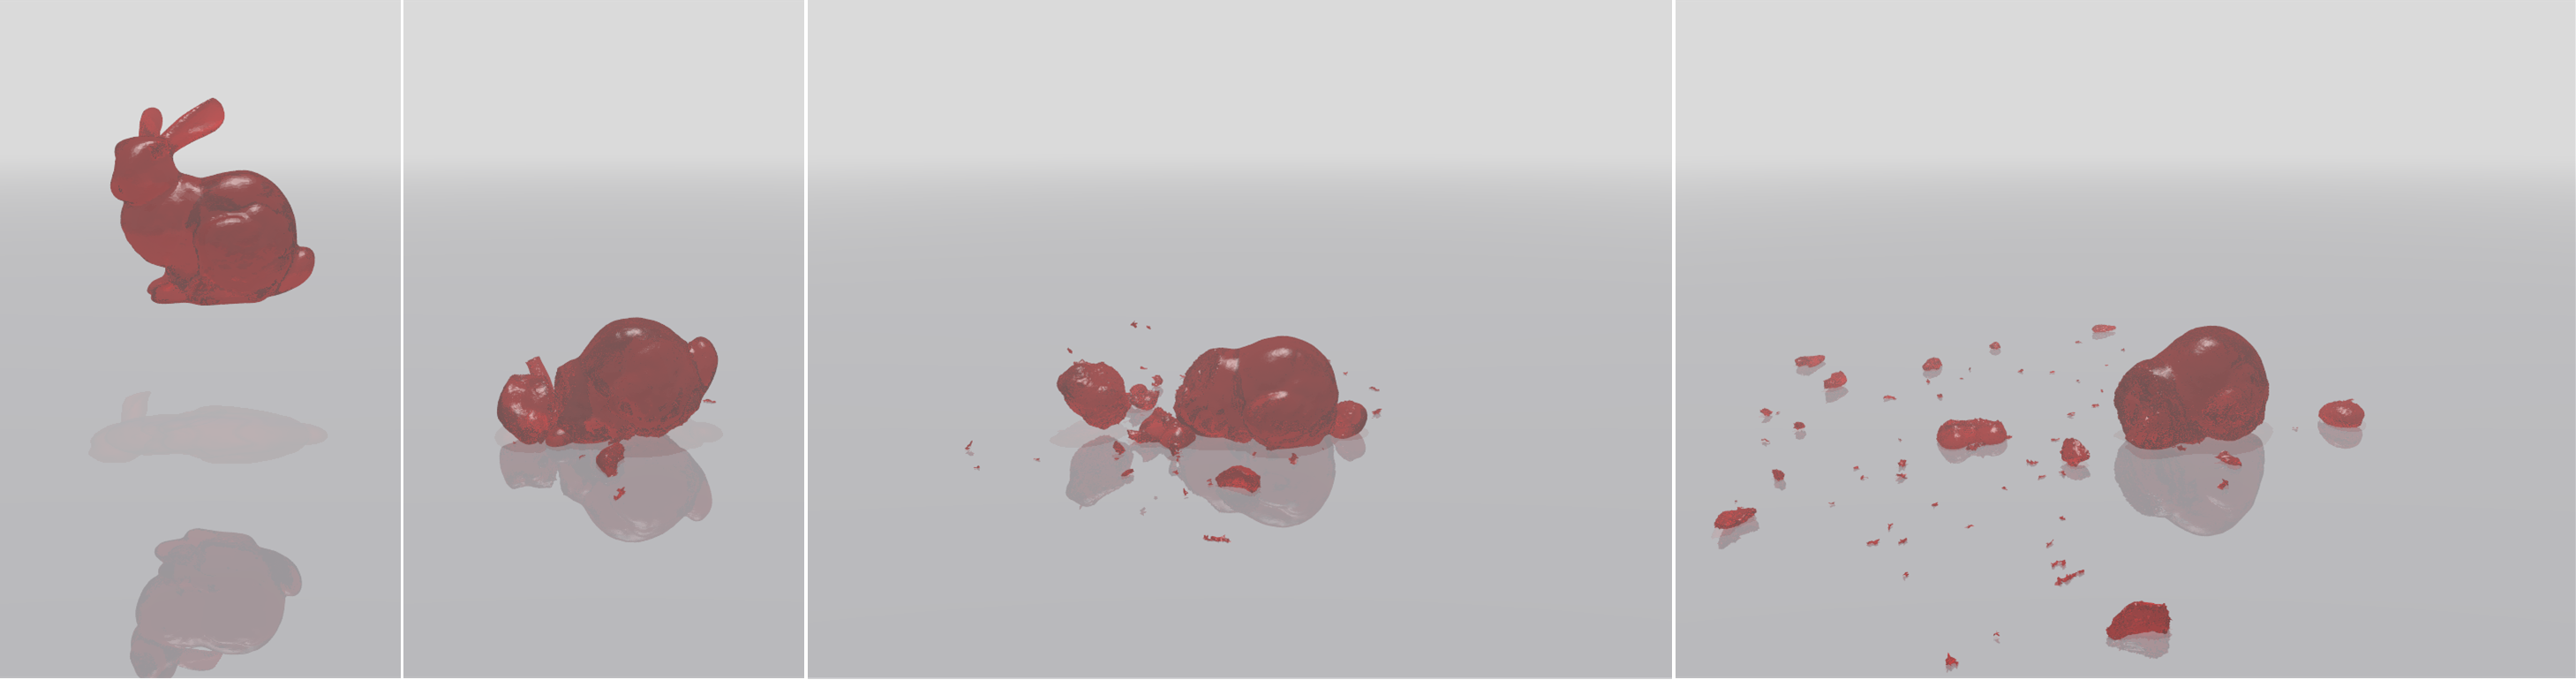
\includegraphics[width=\linewidth]{../figs/demo_fall_bunny.png}
  \caption{\label{fig:15}
  An elastic bunny falls to the ground and shatters into pieces. Note the secondary fracture of the fragments.
}
\end{figure*}
\begin{figure}[t]
  \centering
  %\mbox{} \hfill
  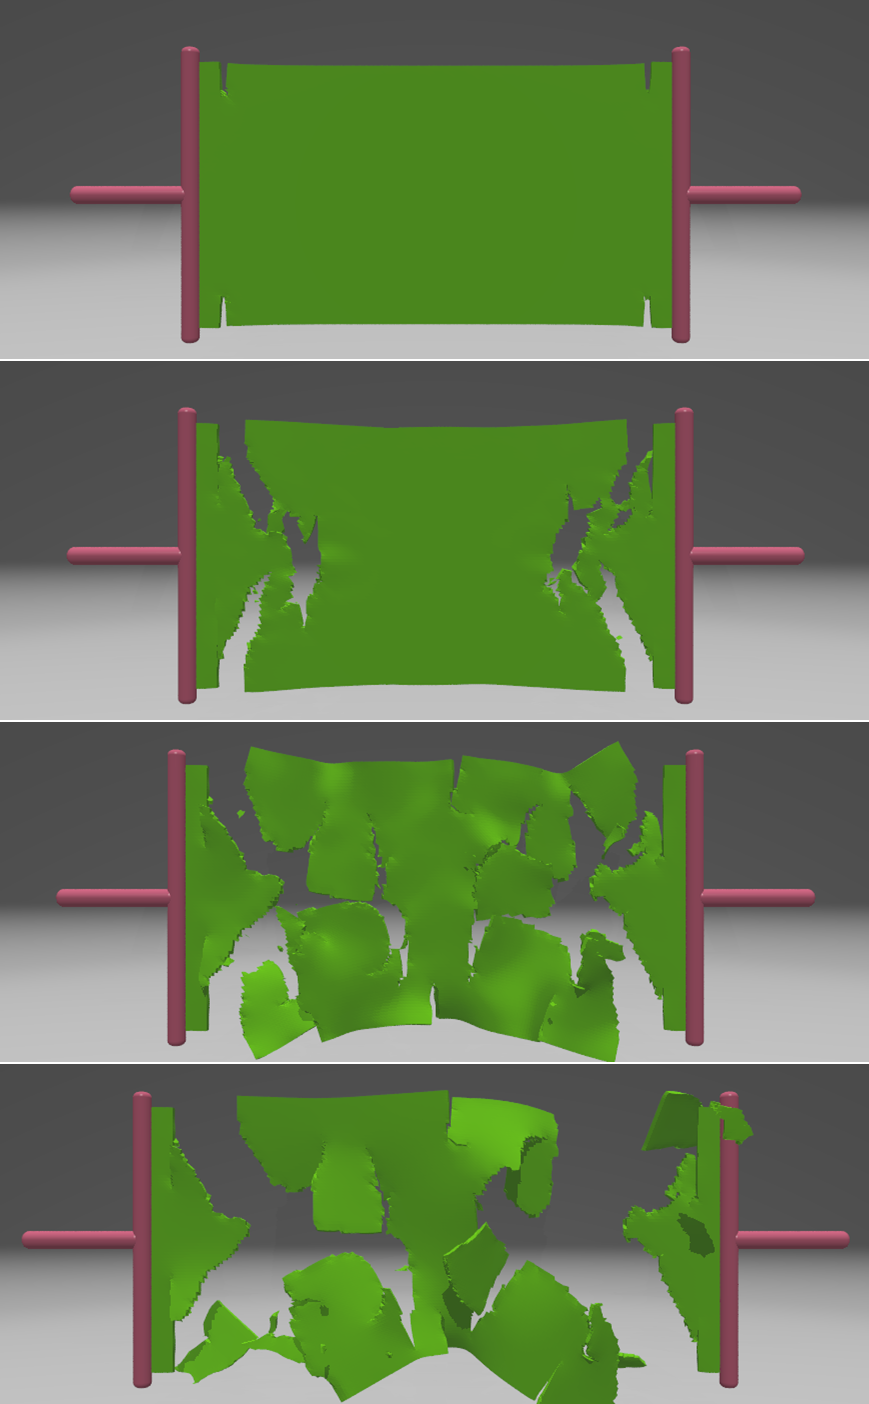
\includegraphics[width=\linewidth]{../figs/revision/demo_tear_thin_sheet.png}
  \caption{\label{fig:16}
  A thin sheet with initial cracks is torn apart. The cracks proceed with branching and merging, separating the sheet into pieces.
}
\end{figure}
\begin{figure}[t]
  \centering
  %\mbox{} \hfill
  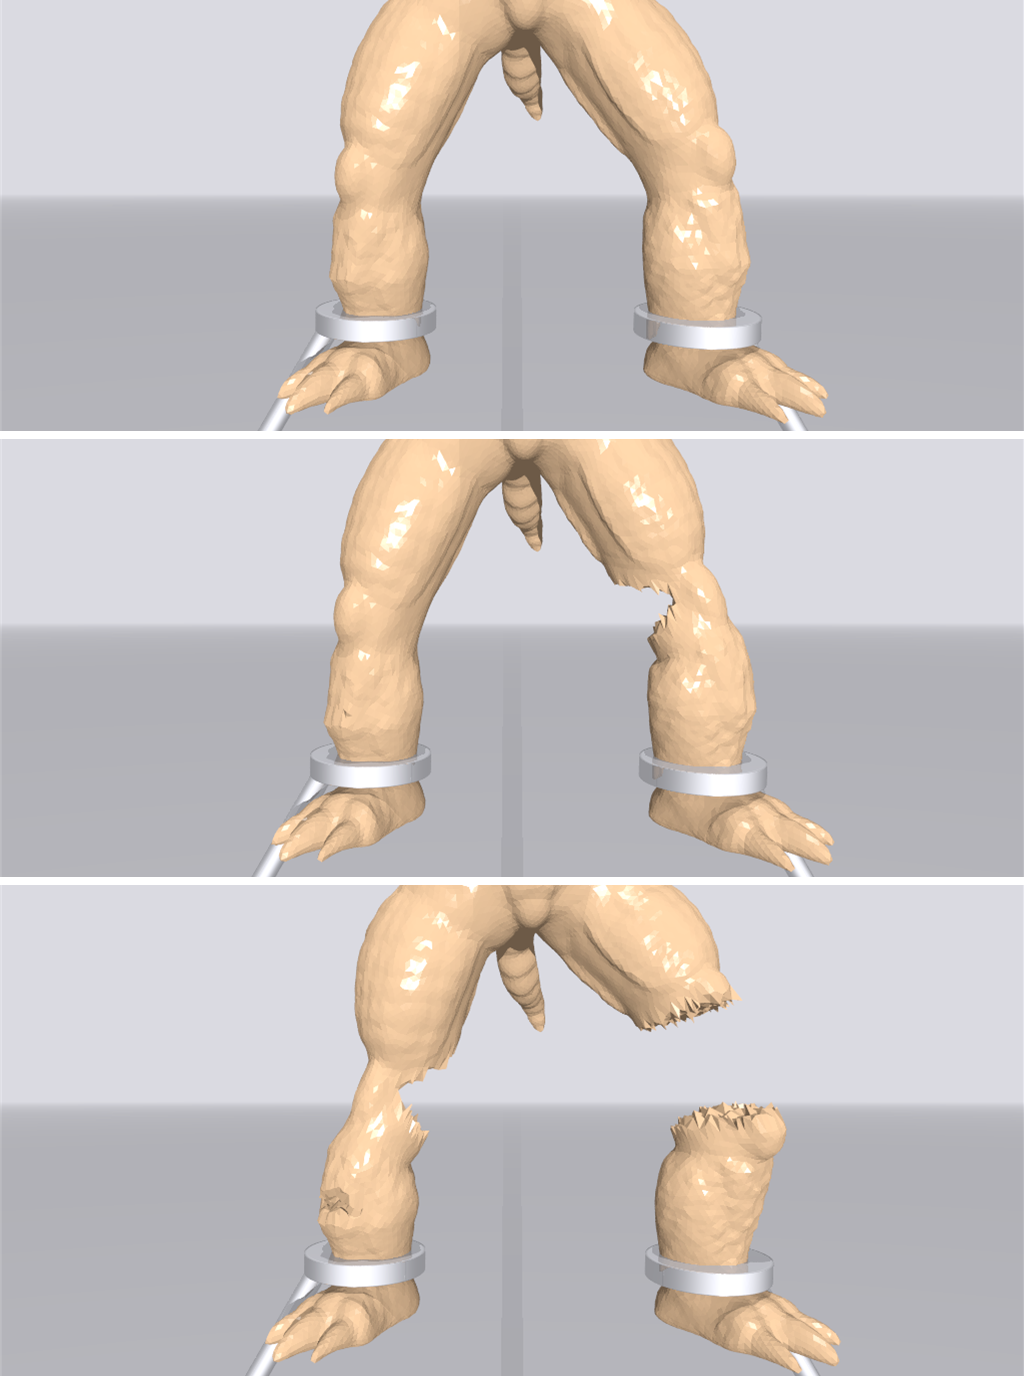
\includegraphics[width=\linewidth]{../figs/demo_tear_armadillo_close_view.png}
  \caption{\label{fig:17}
  A close view of the progressive fracture of the armadillo's legs.
}
\end{figure}
%-------------------------------------------------------------------------
\bibliographystyle{eg-alpha}
%\bibliographystyle{eg-alpha-doi}

\bibliography{../references}

%-------------------------------------------------------------------------
%\newpage

\end{document}
